%%%%%%%%%%%%%%%%%%%%%%%%%%%%% Thesis.tex %%%%%%%%%%%%%%%%%%%%%%%%%%%%%%%
%                                                                      %
%  ---------- Master of Science Dissertation template ----------       %
%                                                                      %
%  Template for the Master Thesis according to the regulations         %
%  published by the Scientific Council at IST.                         %
%                                                                      %
%  For up-to-date regulations, please refer to                         %
%  http://cd.ist.utl.pt/files/publico/academicos/guia_dissertacao.pdf  %
%                                                                      %
%       Andre C. Marta                                                 %
%       Area Cientifica de Mecanica Aplicada e Aeroespacial            %
%       Departamento de Engenharia Mecanica                            %
%       Instituto Superior Tecnico                                     %
%       Av. Rovisco Pais                                               %
%       1049-001 Lisboa                                                %
%       Portugal                                                       %
%       Tel: +351 21 841 9466                                          %
%                        3466 (extension)                              %
%       Email: andre.marta@ist.utl.pt                                  %
%                                                                      %
%  Created:       Jan 20, 2011                                         %
%  Last Modified: Jan 24, 2011                                         %
%                                                                      %
%%%%%%%%%%%%%%%%%%%%%%%%%%%%%%%%%%%%%%%%%%%%%%%%%%%%%%%%%%%%%%%%%%%%%%%%
%                                                                      %
% To generate the PDF file, type "make" at the terminal prompt.        %
%                                                                      %
% The IST template LaTeX package was created by the author             %
% and it can be downloaded from:                                       %
% https://fenix.ist.utl.pt/homepage/ist31052/                          %
%                                                                      %
% The external packages can be downloaded from                         %
% the Comprehensive TeX Archive Network at http://www.ctan.org/        %
%                                                                      %
% List of LaTex symbols:                                               %
% http://www.ctan.org/tex-archive/info/symbols/comprehensive/          %
%                                                                      %
% Help with LaTex can be found at                                      %
% http://www.giss.nasa.gov/tools/latex/ltx-2.html                      %
% http://en.wikibooks.org/wiki/LaTeX                                   %
%%%%%%%%%%%%%%%%%%%%%%%%%%%%%%%%%%%%%%%%%%%%%%%%%%%%%%%%%%%%%%%%%%%%%%%%

%%%%%%%%%%%%%%%%%%%%%%%%%%%%%%%%%%%%%%%%%%%%%%%%%%%%%%%%%%%%%%%%%%%%%%%%
%     Preamble                                                         %
%%%%%%%%%%%%%%%%%%%%%%%%%%%%%%%%%%%%%%%%%%%%%%%%%%%%%%%%%%%%%%%%%%%%%%%%

% ----------------------------------------------------------------------
%  Set the document class
% ----------------------------------------------------------------------
\documentclass[10pt,a4paper,twoside]{report}

% ----------------------------------------------------------------------
% Define external packages, language, margins, fonts and new commands
% ----------------------------------------------------------------------
%%%%%%%%%%%%%%%%%%%%%%%%%%%%%%%%%%%%%%%%%%%%%%%%%%%%%%%%%%%%%%%%%%%%%%%%
%                                                                      %
%     File: Thesis_Preamble.tex                                        %
%     Tex Master: Thesis.tex                                           %
%                                                                      %
%     Author: Andre C. Marta                                           %
%     Last modified : 24 Jan 2011                                      %
%                                                                      %
%%%%%%%%%%%%%%%%%%%%%%%%%%%%%%%%%%%%%%%%%%%%%%%%%%%%%%%%%%%%%%%%%%%%%%%%

% ----------------------------------------------------------------------
% Define document language.
% ----------------------------------------------------------------------

% 'inputenc' package
%
% Accept different input encodings.
% http://www.ctan.org/tex-archive/macros/latex/base/
%
% > allows typing non-english text in LaTeX sources.
%
% ******************************* SELECT *******************************
%\usepackage[latin1]{inputenc} % <<<<< Windows
\usepackage[utf8]{inputenc}   % <<<<< Linux
% ******************************* SELECT *******************************


% 'babel' package
%
% Multilingual support for Plain TeX or LaTeX.
% http://www.ctan.org/tex-archive/macros/latex/required/babel/
%
% > sets the variable names according to the language selected
%
% ******************************* SELECT *******************************
%\usepackage[portuguese]{babel} % <<<<< Portuguese
\usepackage[english]{babel} % <<<<< English
% ******************************* SELECT *******************************


% List of LaTeX variable names: \abstractname, \appendixname, \bibname,
%   \chaptername, \contentsname, \listfigurename, \listtablename, ...)
% http://www.tex.ac.uk/cgi-bin/texfaq2html?label=fixnam
%
% Changing the words babel uses (uncomment and redefine as necessary...)
%
\newcommand{\acknowledgments}{@undefined} % new LaTeX variable name
%
% > English
%
\addto\captionsenglish{\renewcommand{\acknowledgments}{Acknowledgments}}
%\addto\captionsenglish{\renewcommand{\listtablename}{List of Tables}}
%\addto\captionsenglish{\renewcommand{\listfigurename}{List of Figures}}
%\addto\captionsenglish{\renewcommand{\nomname}{Nomenclature}}
%\addto\captionsenglish{\renewcommand{\appendixname}{Appendix}}
%\addto\captionsenglish{\renewcommand{\bibname}{References}} % Bibliography

% > Portuguese
%
\addto\captionsportuguese{\renewcommand{\acknowledgments}{Agradecimentos}}
%\addto\captionsportuguese{\renewcommand{\listtablename}{Lista de Figuras}}
%\addto\captionsportuguese{\renewcommand{\listfigurename}{Lista de Tabelas}}
%\addto\captionsportuguese{\renewcommand{\nomname}{Lista de S\'{i}mbolos}} % Nomenclatura
%\addto\captionsportuguese{\renewcommand{\appendixname}{Anexo}} % Apendice
%\addto\captionsportuguese{\renewcommand{\bibname}{Refer\^{e}ncias}} % Bibliografia


% ----------------------------------------------------------------------
% Define default and cover page fonts.
% ----------------------------------------------------------------------

% Use Arial font as default
%
\renewcommand{\rmdefault}{phv}
\renewcommand{\sfdefault}{phv}

% Define cover page fonts
%
%         encoding     family       series      shape
%  \usefont{T1}     {phv}=helvetica  {b}=bold    {n}=normal
%                   {ptm}=times      {m}=normal  {sl}=slanted
%                                                {it}=italic
% see more examples at
% http://julien.coron.free.fr/languages/latex/fonts/
%
\def\FontLn{% 16 pt normal
  \usefont{T1}{phv}{m}{n}\fontsize{16pt}{16pt}\selectfont}
\def\FontLb{% 16 pt bold
  \usefont{T1}{phv}{b}{n}\fontsize{16pt}{16pt}\selectfont}
\def\FontMn{% 14 pt normal
  \usefont{T1}{phv}{m}{n}\fontsize{14pt}{14pt}\selectfont}
\def\FontMb{% 14 pt bold
  \usefont{T1}{phv}{b}{n}\fontsize{14pt}{14pt}\selectfont}
\def\FontSn{% 12 pt normal
  \usefont{T1}{phv}{m}{n}\fontsize{12pt}{12pt}\selectfont}


% ----------------------------------------------------------------------
% Define page margins and line spacing.
% ----------------------------------------------------------------------

% 'geometry' package
%
% Flexible and complete interface to document dimensions.
% http://www.ctan.org/tex-archive/macros/latex/contrib/geometry/
%
% > set the page margins (2.5cm minimum in every side, as per IST rules)
%
\usepackage{geometry}	
\geometry{verbose,tmargin=2.5cm,bmargin=2.5cm,lmargin=2.5cm,rmargin=2.5cm}

% 'setspace' package
%
% Set space between lines.
% http://www.ctan.org/tex-archive/macros/latex/contrib/setspace/
%
% > allow setting line spacing (line spacing of 1.5, as per IST rules)
%
\usepackage{setspace}
\renewcommand{\baselinestretch}{1.5}


% ----------------------------------------------------------------------
% Include external packages.
% Note that not all of these packages may be available on all system
% installations. If necessary, include the .sty files locally in
% the <jobname>.tex file directory.
% ----------------------------------------------------------------------

% 'graphicx' package
%
% Enhanced support for graphics.
% http://www.ctan.org/tex-archive/macros/latex/required/graphics/
%
% > extends arguments of the \includegraphics command
%
\usepackage{graphicx}


% 'color' package
%
% Colour control for LaTeX documents.
% http://www.ctan.org/tex-archive/macros/latex/required/graphics/
%
% > defines color macros: \color{<color name>}
%
%\usepackage{color}


% 'amsmath' package
%
% Mathematical enhancements for LaTeX.
% http://www.ctan.org/tex-archive/macros/latex/required/amslatex/
%
% > American Mathematical Society plain Tex macros
%
\usepackage{amsmath}  % AMS mathematical facilities for LaTeX.
\usepackage{amsthm}   % Typesetting theorems (AMS style).
\usepackage{amsfonts} % 


% 'wrapfig' package
%
% Produces figures which text can flow around.
% http://www.ctan.org/tex-archive/macros/latex/contrib/wrapfig/
%
% > wrap figures/tables in text (i.e., Di Vinci style)
%
% \usepackage{wrapfig}


% 'subfigure' package
%
% Deprecated: Figures divided into subfigures.
% http://www.ctan.org/tex-archive/obsolete/macros/latex/contrib/subfigure/
%
% > subcaptions for subfigures
%
\usepackage{subfigure}


% 'subfigmat' package
%
% Automates layout when using the subfigure package.
% http://www.ctan.org/tex-archive/macros/latex/contrib/subfigmat/
%
% > matrices of similar subfigures
%
\usepackage{subfigmat}


% 'url' package
%
% Verbatim with URL-sensitive line breaks.
% http://www.ctan.org/tex-archive/macros/latex/contrib/url/
%
% > URLs in BibTex
%
% \usepackage{url}


% 'varioref' package
%
% Intelligent page references.
% http://www.ctan.org/tex-archive/macros/latex/required/tools/
%
% > smart page, figure, table and equation referencing
%
%\usepackage{varioref}


% 'dcolumn' package
%
% Align on the decimal point of numbers in tabular columns.
% http://www.ctan.org/tex-archive/macros/latex/required/tools/
%
% > decimal-aligned tabular math columns
%
\usepackage{dcolumn}
\newcolumntype{d}{D{.}{.}{-1}} % column aligned by the point separator '.'
\newcolumntype{e}{D{E}{E}{-1}} % column aligned by the exponent 'E'


% '' package
%
% Reimplementation of and extensions to LaTeX verbatim.
% http://www.ctan.org/tex-archive/macros/latex/required/tools/
%
% > provides the verbatim environment (\begin{verbatim},\end{verbatim})
%   and a comment environment (\begin{comment},  \end{comment})
%
% \usepackage{verbatim}


% 'moreverb' package
%
% Extended verbatim.
% http://www.ctan.org/tex-archive/macros/latex/contrib/moreverb/
%
% > supports tab expansion and line numbering
%
% \usepackage{moreverb}



% 'nomencl' package
%
% Produce lists of symbols as in nomenclature.
% http://www.ctan.org/tex-archive/macros/latex/contrib/nomencl/
%
% The nomencl package makes use of the MakeIndex program
% in order to produce the nomenclature list.
%
% Nomenclature
% 1) On running the file through LATEX, the command \makenomenclature
%    in the preamble instructs it to create/open the nomenclature file
%    <jobname>.nlo corresponding to the LATEX file <jobname>.tex and
%    writes the information from the \nomenclature commands to this file.
% 2) The next step is to invoke MakeIndex in order to produce the
%    <jobname>.nls file. This can be achieved by making use of the
%    command: makeindex <jobname>.nlo -s nomencl.ist -o <jobname>.nls
% 3) The last step is to invoke LATEX on the <jobname>.tex file once
%    more. There, the \printnomenclature in the document will input the
%    <jobname>.nls file and process it according to the given options.
%
% http://www-h.eng.cam.ac.uk/help/tpl/textprocessing/nomencl.pdf
%
\usepackage{nomencl}
\makenomenclature
%
% Group variables according to their symbol type
%
\RequirePackage{ifthen} 
\ifthenelse{\equal{\languagename}{english}}%
    { % English
    \renewcommand{\nomgroup}[1]{%
      \ifthenelse{\equal{#1}{R}}{%
        \item[\textbf{Roman symbols}]}{%
        \ifthenelse{\equal{#1}{G}}{%
          \item[\textbf{Greek symbols}]}{%
          \ifthenelse{\equal{#1}{S}}{%
            \item[\textbf{Subscripts}]}{%
            \ifthenelse{\equal{#1}{T}}{%
              \item[\textbf{Superscripts}]}{}}}}}%
    }{% Portuguese
    \renewcommand{\nomgroup}[1]{%
      \ifthenelse{\equal{#1}{R}}{%
        \item[\textbf{Simbolos romanos}]}{%
        \ifthenelse{\equal{#1}{G}}{%
          \item[\textbf{Simbolos gregos}]}{%
          \ifthenelse{\equal{#1}{S}}{%
            \item[\textbf{Subscritos}]}{%
            \ifthenelse{\equal{#1}{T}}{%
              \item[\textbf{Sobrescritos}]}{}}}}}%
    }%


%
% Acronimos
%
\usepackage{acronym} 



% 'rotating' package
%
% Rotation tools, including rotated full-page floats.
% http://www.ctan.org/tex-archive/macros/latex/contrib/rotating/
%
% > show wide figures and tables in landscape format:
%   use \begin{sidewaystable} and \begin{sidewaysfigure}
%   instead of 'table' and 'figure', respectively.
%
\usepackage{rotating}


% 'hyperref' package
%
% Extensive support for hypertext in LaTeX.
% http://www.ctan.org/tex-archive/macros/latex/contrib/hyperref/
%
% > Extends the functionality of all the LATEX cross-referencing
%   commands (including the table of contents, bibliographies etc) to
%   produce \special commands which a driver can turn into hypertext
%   links; Also provides new commands to allow the user to write adhoc
%   hypertext links, including those to external documents and URLs.
%
\usepackage[pdftex]{hyperref} % enhance documents that are to be
                              % output as HTML and PDF
\hypersetup{colorlinks,       % color text of links and anchors,
                              % eliminates borders around links
%            linkcolor=red,    % color for normal internal links
            linkcolor=black,  % color for normal internal links
            anchorcolor=black,% color for anchor text
%            citecolor=green,  % color for bibliographical citations
            citecolor=black,  % color for bibliographical citations
%            filecolor=magenta,% color for URLs which open local files
            filecolor=black,  % color for URLs which open local files
%            menucolor=red,    % color for Acrobat menu items
            menucolor=black,  % color for Acrobat menu items
%            pagecolor=red,    % color for links to other pages
%            pagecolor=black,  % color for links to other pages
%            urlcolor=cyan,    % color for linked URLs
            urlcolor=black,   % color for linked URLs
	          bookmarks=true,         % create PDF bookmarks
	          bookmarksopen=false,    % don't expand bookmarks
	          bookmarksnumbered=true, % number bookmarks
	          pdftitle={Thesis},
            pdfauthor={Carlos E. H. J. Fonseca},
            pdfsubject={Eagle Eye},
            pdfkeywords={},
            pdfstartview=FitV,
            pdfdisplaydoctitle=true}


% 'hypcap' package
%
% Adjusting the anchors of captions.
% http://www.ctan.org/tex-archive/macros/latex/contrib/oberdiek/
%
% > fixes the problem with hyperref, that links to floats points
%   below the caption and not at the beginning of the float.
%
\usepackage[figure,table]{hypcap}


% 'natbib' package
%
% Flexible bibliography support.
% http://www.ctan.org/tex-archive/macros/latex/contrib/natbib/
%
% > produce author-year style citations
%
% \citet  and \citep  for textual and parenthetical citations, respectively
% \citet* and \citep* that print the full author list, and not just the abbreviated one
% \citealt is the same as \citet but without parentheses. Similarly, \citealp is \citep without parentheses
% \citeauthor
% \citeyear
% \citeyearpar
%
%\usepackage{natbib}


% ----------------------------------------------------------------------
% Define new commands to assure consistent treatment throughout document
% ----------------------------------------------------------------------

\newcommand{\ud}{\mathrm{d}}                % total derivative
\newcommand{\degree}{\ensuremath{^\circ\,}} % degrees

% Abbreviations

\newcommand{\mcol}{\multicolumn}            % table format

\newcommand{\eqnref}[1]{(\ref{#1})}
\newcommand{\class}[1]{\texttt{#1}}
\newcommand{\package}[1]{\texttt{#1}}
\newcommand{\file}[1]{\texttt{#1}}
\newcommand{\BibTeX}{\textsc{Bib}\TeX}

% Typefaces ( example: {\bf Bold text here} )
%
% > pre-defined
%   \bf % bold face
%   \it % italic
%   \tt % typewriter
%
% > newly defined
\newcommand{\tr}[1]{{\ensuremath{\textrm{#1}}}}   % text roman
\newcommand{\tb}[1]{{\ensuremath{\textbf{#1}}}}   % text bold face
\newcommand{\ti}[1]{{\ensuremath{\textit{#1}}}}   % text italic
\newcommand{\mc}[1]{{\ensuremath{\mathcal{#1}}}}  % math calygraphy
\newcommand{\mco}[1]{{\ensuremath{\mathcalold{#1}}}}% math old calygraphy
\newcommand{\mr}[1]{{\ensuremath{\mathrm{#1}}}}   % math roman
\newcommand{\mb}[1]{{\ensuremath{\mathbf{#1}}}}   % math bold face
\newcommand{\bs}[1]{\ensuremath{\boldsymbol{#1}}} % math symbol
\def\bm#1{\mathchoice                             % math bold
  {\mbox{\boldmath$\displaystyle#1$}}%
  {\mbox{\boldmath$#1$}}%
  {\mbox{\boldmath$\scriptstyle#1$}}%
  {\mbox{\boldmath$\scriptscriptstyle#1$}}}
\newcommand{\boldcal}[1]{{\ensuremath{\boldsymbol{\mathcal{#1}}}}}% math bold calygraphy

\usepackage{pdflscape} %Paginas na Horizontal
\usepackage{array}	% Tables
\usepackage{multirow} %Colunas grandes em tabelas
\usepackage{bbding} % checkmarks and other symbols

% My Commands

\usepackage{wrapfig}
\usepackage{listings}
\usepackage{epigraph}

\usepackage[table]{xcolor}

\renewcommand{\thesubfigure}{\thefigure.\arabic{subfigure}}
\makeatletter
\renewcommand{\p@subfigure}{}
\renewcommand{\@thesubfigure}{\thesubfigure:\hskip\subfiglabelskip}
\makeatother


\newenvironment{enum}{
	\begin{enumerate}
	  \setlength{\itemsep}{1pt}
	  \setlength{\parskip}{0pt}
	  \setlength{\parsep}{0pt}}{
	\end{enumerate}
}

\newenvironment{myitemize}{
	\begin{itemize}
	  \setlength{\itemsep}{1pt}
	  \setlength{\parskip}{0pt}
	  \setlength{\parsep}{0pt}}{
	\end{itemize}
}

\newcommand{\hide}[1]{}
\newcommand{\super}[1]{\ensuremath{^{\textrm{#1}}}}
\newcommand{\fig}[1]{fig. \ref{fig:#1}}
\newcommand{\Fig}[1]{Fig. \ref{fig:#1}}
\newcommand{\cm}{\Checkmark}
\newcommand{\todo}[1]{\textcolor{red}{TODO: #1}}
\newcommand{\red}[1]{\textcolor{red}{#1}}
\newcommand{\refs}{\todo{References needed} }

\definecolor{light-gray}{gray}{0.92}
 % file "Thesis_Preamble.tex"

%%%%%%%%%%%%%%%%%%%%%%%%%%%%%%%%%%%%%%%%%%%%%%%%%%%%%%%%%%%%%%%%%%%%%%%%
%     Begin Document                                                   %
%%%%%%%%%%%%%%%%%%%%%%%%%%%%%%%%%%%%%%%%%%%%%%%%%%%%%%%%%%%%%%%%%%%%%%%%
\begin{document}

% Set plain page style (no headers, footer with centered page number)
\pagestyle{plain}

% Set roman numbering (i,ii,...) before the start of chapters
\pagenumbering{roman}

% ----------------------------------------------------------------------
%  Cover page
% ----------------------------------------------------------------------
%!TEX root = /Users/carlos/Dropbox/Tese/Disertação/Thesis.tex
%%%%%%%%%%%%%%%%%%%%%%%%%%%%%%%%%%%%%%%%%%%%%%%%%%%%%%%%%%%%%%%%%%%%%%%%
%                                                                      %
%     File: Thesis_FrontCover.tex                                      %
%     Tex Master: Thesis.tex                                           %
%                                                                      %
%     Author: Andre C. Marta                                           %
%     Last modified : 21 Jan 2011                                      %
%                                                                      %
%%%%%%%%%%%%%%%%%%%%%%%%%%%%%%%%%%%%%%%%%%%%%%%%%%%%%%%%%%%%%%%%%%%%%%%%

\thispagestyle {empty}

% IST Logo
% parameters: bb=llx lly urx ury (bounding box), width=h_length, height=v_length, angle=angle, scale=factor, clip=true/false, draft=true/false. 

\includegraphics[bb=1.86cm 0cm 10cm 3.16cm,scale=0.56]{Logo}

\begin{center}
%
% Figure (Image or plot)
\vspace{6cm}
%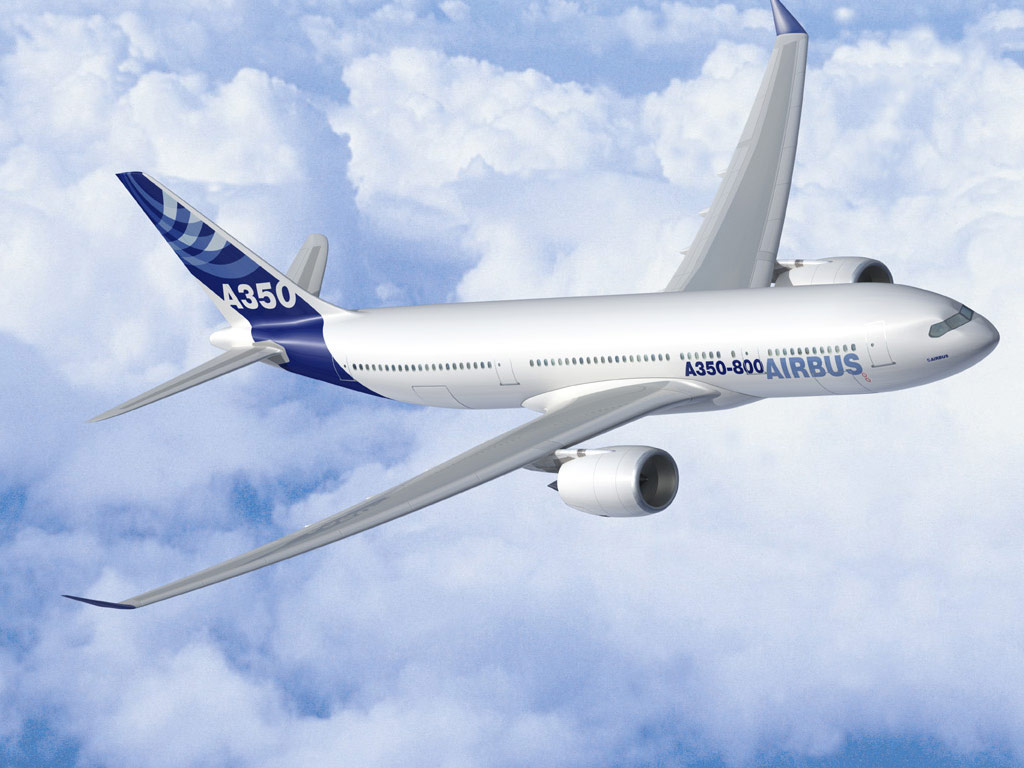
\includegraphics[height=50mm]{Figures/Airbus_A350.jpg}

% Title, author and degree
\vspace{0.8cm}
{\FontLb EagleEye} \\
\vspace{0.2cm}
{\FontMn Large photoset visualization } \\
\vspace{1.9cm}
{\FontMb Carlos Eduardo Henriques de Jesus Fonseca} \\
\vspace{1.9cm}
{\FontLn Disserta\c{c}\~{a}o para a obten\c{c}\~{a}o de Grau de Mestre em} \\
\vspace{0.3cm}
{\FontLb Engenharia Informática e de Computadores} \\
\vspace{1.9cm}
{\FontMb J\'{u}ri} \\
\vspace{0.3cm}
{\FontSn %
\begin{tabular}{ll}
Presidente: & Nome do Presidente \\
Orientador: & Nome do Orientador \\
Co-orientador: & Nome do Co-orientador \\
Vogais: & Nome do Vogal 1 \\
        & Nome do Vogal 2 \\
        & Nome do Vogal 3 \\
\end{tabular} } \\
\vspace{1.1cm}
{\FontMb M\^{e}s e Ano} \\
%
\end{center}

\cleardoublepage

 % file "Thesis_FrontCover.tex"

% ----------------------------------------------------------------------
% Dedication page (optional)
% ----------------------------------------------------------------------
%%%%%%%%%%%%%%%%%%%%%%%%%%%%%%%%%%%%%%%%%%%%%%%%%%%%%%%%%%%%%%%%%%%%%%%%
%                                                                      %
%     File: Thesis_Dedication.tex                                      %
%     Tex Master: Thesis.tex                                           %
%                                                                      %
%     Author: Andre C. Marta                                           %
%     Last modified : 21 Jan 2011                                      %
%                                                                      %
%%%%%%%%%%%%%%%%%%%%%%%%%%%%%%%%%%%%%%%%%%%%%%%%%%%%%%%%%%%%%%%%%%%%%%%%

\null\vskip5cm%
\begin{flushright}
     \red{Dedicated to someone special...}
\end{flushright}
\vfill\newpage

\cleardoublepage

 % file "Thesis_Dedication.tex"

% ----------------------------------------------------------------------
%  Acknowledgments (optional)
% ----------------------------------------------------------------------
%%%%%%%%%%%%%%%%%%%%%%%%%%%%%%%%%%%%%%%%%%%%%%%%%%%%%%%%%%%%%%%%%%%%%%%%
%                                                                      %
%     File: Thesis_Acknowledgments.tex                                 %
%     Tex Master: Thesis.tex                                           %
%                                                                      %
%     Author: Andre C. Marta                                           %
%     Last modified : 21 Jan 2011                                      %
%                                                                      %
%%%%%%%%%%%%%%%%%%%%%%%%%%%%%%%%%%%%%%%%%%%%%%%%%%%%%%%%%%%%%%%%%%%%%%%%

\section*{\acknowledgments}

% Add entry in the table of contents as section
\addcontentsline{toc}{section}{\acknowledgments}

\red{A few words about the university, financial support, research advisor, dissertation readers, faculty or other professors, lab mates, other friends and family...
}

\cleardoublepage

 % file "Thesis_Acknowledgements.tex"

% ----------------------------------------------------------------------
%  Abstract (both in English and Portuguese)
% ----------------------------------------------------------------------
%%%%%%%%%%%%%%%%%%%%%%%%%%%%%%%%%%%%%%%%%%%%%%%%%%%%%%%%%%%%%%%%%%%%%%%%
%                                                                      %
%     File: Thesis_Resumo.tex                                          %
%     Tex Master: Thesis.tex                                           %
%                                                                      %
%     Author: Andre C. Marta                                           %
%     Last modified : 21 Jan 2011                                      %
%                                                                      %
%%%%%%%%%%%%%%%%%%%%%%%%%%%%%%%%%%%%%%%%%%%%%%%%%%%%%%%%%%%%%%%%%%%%%%%%

\chapter*{Resumo e palavras chave}

% Add entry in the table of contents as section
\addcontentsline{toc}{section}{Resumo e palavras chave}

A fotografia digital tem feito parte da vida das pessoas na ultima década, crescendo nos discos rígidos, mas a visualização de imagens não tem vindo a evoluir o suficiente para acompanhar este crescimento. A maior parte das pessoas guarda as fotos em pastas ou utiliza programas que não conseguem mostrar grandes quantidades de fotografias ao mesmo tempo, não fornecendo uma visão global da biblioteca.

Este trabalho cresceu das características de outros trabalhos de visualizações alternativas de imagens e tenta trazer a utilizadores comuns uma melhor maneira de explorar as suas bibliotecas de fotografias e aprender mais sobre elas.

Este trabalho fornece um sistema extensível para a extracção e agregação de características das imagens do utilizador e respectivos meta-dados, Actualmente são extraidas cores, rostos, datas, pastas e palavras-chave, mas, já que é extensível, poderá ser utilizado para muito mais.

Também criámos uma aplicação de visualização que usa os dados processados e os disponibiliza aos utilizadores numa interface limpa e simples. A aplicação começa por apresentar no ecrã, numa grelha, todas as imagens adicionadas ao programa, agrupados por datas. A partir daqui, o utilizador pode alterar a visualização ampliando-a ou reduzindo-a, organizando as imagens por cores, rostos ou pastas, podendo ainda filtrar utilizando uma mistura de todos os dados recolhidos pelo sistema de processamento. Desta forma, os utilizadores podem visualizar e explorar suas bibliotecas de uma forma diferente daquilo a que estão habituados.

\vfill

\textbf{Palavras-chave:} fotografias, visualização de imagens, exploração de imagens, extração de caracteristicas

\cleardoublepage

 % file "Thesis_Resumo.tex"
%%%%%%%%%%%%%%%%%%%%%%%%%%%%%%%%%%%%%%%%%%%%%%%%%%%%%%%%%%%%%%%%%%%%%%%%
%                                                                      %
%     File: Thesis_Abstract.tex                                        %
%     Tex Master: Thesis.tex                                           %
%                                                                      %
%     Author: Andre C. Marta                                           %
%     Last modified : 21 Jan 2011                                      %
%                                                                      %
%%%%%%%%%%%%%%%%%%%%%%%%%%%%%%%%%%%%%%%%%%%%%%%%%%%%%%%%%%%%%%%%%%%%%%%%

\chapter*{Abstract and keywords}

% Add entry in the table of contents as section
\addcontentsline{toc}{section}{Abstract and keywords}

\red{Insert your abstract here with a maximum of 250 words, followed by 4 to 6 keywords...
}
\vfill

\textbf{Keywords:} \red{photographs, image visualization, image browsing},...

\cleardoublepage

 % file "Thesis_Abstract.tex"

% ----------------------------------------------------------------------
%  Table of contents, list of tables, list of figures and nomenclature
% ----------------------------------------------------------------------

% Table of contents
%
\tableofcontents
\cleardoublepage 

% List of tables
%
% Generate list
\listoftables
% Add entry in the table of contents as section
\addcontentsline{toc}{section}{\listtablename}
\cleardoublepage 

% List of figures
%
% Generate list
\listoffigures
% Add entry in the table of contents as section
\addcontentsline{toc}{section}{\listfigurename}
\cleardoublepage 

% Nomenclature
%
% entries of nomenclature list
\addcontentsline{toc}{section}{Acronyms}
%%%%%%%%%%%%%%%%%%%%%%%%%%%%%%%%%%%%%%%%%%%%%%%%%%%%%%%%%%%%%%%%%%%%%%%%
%                                                                      %
%     File: Thesis_Nomenclature.tex                                    %
%     Tex Master: Thesis.tex                                           %
%                                                                      %
%     Author: Andre C. Marta                                           %
%     Last modified : 21 Jan 2011                                      %
%                                                                      %
%%%%%%%%%%%%%%%%%%%%%%%%%%%%%%%%%%%%%%%%%%%%%%%%%%%%%%%%%%%%%%%%%%%%%%%%
%
% The definitions can be placed anywhere in the document body
% and their order is sorted by <symbol> automatically when
% calling makeindex in the makefile
%
% The \glossary command has the following syntax:
%
% \glossary{entry}
%
% The \nomenclature command has the following syntax:
%
% \nomenclature[<prefix>]{<symbol>}{<description>}
%
% where <prefix> is used for fine tuning the sort order,
% <symbol> is the symbol to be described, and <description> is
% the actual description.

% ----------------------------------------------------------------------

\chapter*{Acronyms}

% Add entry in the table of contents as section
\addcontentsline{toc}{section}{Acronyms}

\begin{acronym}[TDMA]

\acro{UI}[UI]{user interface}
\acro{UX}[UX]{user experience}
\acro{SOM}[SOM]{self organizing map}
\acro{CBIR}[CBIR]{content based image retrieval}
\acro{MP}[MP]{megapixel}
\acro{FEP}[FEP]{feature extraction plugin}
\acro{WPF}[WPF]{Windows Presentation Foundation}
\acro{EXIF}[EXIF]{Exchangeable image file format}
\acro{HDR}[HDR]{High Dynamic Range}

\end{acronym}
\vfill

\cleardoublepage % file "Thesis_Nomenclature.tex"
%
% Insert glossary/nomenclature section produced by MakeIndex
%\printnomenclature
% Add entry in the table of contents as section
\addcontentsline{toc}{section}{\nomname}
\cleardoublepage

% Set arabic numbering (1,2,...) after preface
%

\setcounter{page}{1}
\pagenumbering{arabic}

% ----------------------------------------------------------------------
%  Chapters
% ----------------------------------------------------------------------

%%%%%%%%%%%%%%%%%%%%%%%%%%%%%%%%%%%%%%%%%%%%%%%%%%%%%%%%%%%%%%%%%%%%%%%%%
%                                                                      %
%     File: Thesis_Introduction.tex                                    %
%     Tex Master: Thesis.tex                                           %
%                                                                      %
%     Author: Andre C. Marta                                           %
%     Last modified : 21 Jan 2011                                      %
%                                                                      %
%%%%%%%%%%%%%%%%%%%%%%%%%%%%%%%%%%%%%%%%%%%%%%%%%%%%%%%%%%%%%%%%%%%%%%%%

\chapter{Stuff}
\label{chapter:introduction}

Insert your chapter material here...

% ----------------------------------------------------------------------
\section{Motivation}
\label{section:motivation}

Relevance of the subject...


% ----------------------------------------------------------------------
\section{State-of-the-art}
\label{section:state}

Insert your section material with the appropriate citations.
These can be cited in the following way: \\

Citation mode \#1 - \quad \cite{jameson:adjointns}
Citation mode \#2 - \quad \citet{jameson:adjointns}
Citation mode \#3 - \quad \citep{jameson:adjointns}
Citation mode \#4 - \quad \citet*{jameson:adjointns}
Citation mode \#5 - \quad \citep*{jameson:adjointns}
Citation mode \#6 - \quad \citealt{jameson:adjointns}
Citation mode \#7 - \quad \citealp{jameson:adjointns}
Citation mode \#8 - \quad \citeauthor{jameson:adjointns}
Citation mode \#9 - \quad \citeyear{jameson:adjointns}
Citation mode \#10 - \quad \citeyearpar{jameson:adjointns}

1	Jameson et al. [1998]
2	Jameson et al. [1998]
3	[Jameson et al., 1998]
4	Jameson, Pierce, and Martinelli [1998]
5	[Jameson, Pierce, and Martinelli, 1998]
6	Jameson et al. 1998
7	Jameson et al.,
8	1998 Jameson et al.
9	1998
10	[1998]


\subsection{Tables}
\label{subsection:tables}

Insert your subsection material and for instance a few tables...

\begin{table}[h!]
  \begin{center}
    \begin{tabular}{|c|c|}
      \hline
      item 1 & item 2 \\
      \hline
      item 3 & item 4 \\
      \hline
    \end{tabular}
  \end{center}
  \caption[Table caption shown in TOC]{Table caption}
  \label{table:simple}
\end{table}

Make reference to Table \ref{table:simple}.

\begin{table}[!htb]
  \begin{center}
    \begin{tabular}{lccc}
      Model           & $C_L$ & $C_D$ & $C_{M y}$ \\
      \hline
      Euler           & 0.083 & 0.021 & -0.110    \\
      Navier--Stokes  & 0.078 & 0.023 & -0.101    \\
      \hline
    \end{tabular}
  \end{center}
  \caption{Aerodynamic coefficients.}
  \label{tab:aeroCoeff}
\end{table}

Here is an example of a table with merging columns:

\begin{table}[!htb]
  \begin{center}
    \begin{tabular}[]{lrr}
      \hline
                     & \multicolumn{2}{c}{\underline{Virtual memory [MB]}} \\
                     & Euler       & Navier--Stokes \\
      \hline
      Wing only      &  1,000      &    2,000       \\
      Aircraft       &  5,000      &   10,000       \\
      (ratio)        & $5.0\times$ & $5.0\times$    \\
      \hline
    \end{tabular}
  \end{center}
  \caption{Memory usage comparison (in MB).}
  \label{tab:memory}
\end{table}


\subsection{Drawings}
\label{subsection:drawings}

Insert your subsection material and for instance a few drawings...

The schematic illustrated in Fig.~\ref{fig:algorithm} can represent some sort of algorithm.

\begin{figure}[!htb]
  \centering
  \scriptsize
%  \footnotesize 
%  \small
  \setlength{\unitlength}{0.9cm}
  \begin{picture}(8.5,6)
    \linethickness{0.3mm}

    \put(3,6){\vector(0,-1){1}}
    \put(3.5,5.4){$\bf \alpha$}
    \put(3,4.5){\oval(6,1){}}
    %\put(0,4){\framebox(6,1){}}
    \put(0.3,4.4){Grid Generation: \quad ${\bf x} = {\bf x}\left({\bf \alpha}\right)$}

    \put(3,4){\vector(0,-1){1}}
    \put(3.5,3.4){$\bf x$}
    \put(3,2.5){\oval(6,1){}}
    %\put(0,2){\framebox(6,1){}}
    \put(0.3,2.4){Flow Solver: \quad ${\cal R}\left({\bf x},{\bf q}\left({\bf x}\right)\right) = 0$}

    \put(6.0,2.5){\vector(1,0){1}}
    \put(6.4,3){$Y_1$}

    \put(3,2){\vector(0,-1){1}}
    \put(3.5,1.4){$\bf q$}
    \put(3,0.5){\oval(6,1){}}
    %\put(0,0){\framebox(6,1){}}
    \put(0.3,0.4){Structural Solver: \quad ${\cal M}\left({\bf x},{\bf q}\left({\bf x}\right)\right) = 0$}

    \put(6.0,0.5){\vector(1,0){1}}
    \put(6.4,1){$Y_2$}

    %\put(7.8,2.5){\oval(1.6,5){}}
    \put(7.0,0){\framebox(1.6,5){}}
    \put(7.1,2.5){Optimizer}
    \put(7.8,5){\line(0,1){1}}
    \put(7.8,6){\line(-1,0){4.8}}
  \end{picture}
  \caption{Schematic of some algorithm.}
  \label{fig:algorithm}
\end{figure}

\cleardoublepage



\chapter{Introduction} % 5/6 pages
\label{chapter:introduction}


% \section{Prologue} % (fold)
% \label{sec:prologue}

\setlength{\epigraphwidth}{.5\textwidth}
\setlength{\afterepigraphskip}{\baselineskip}

\epigraph{\emph{\textbf{photography}}\newline
noun\newline
the art or practice of taking and processing photographs.}{\footnotesize New Oxford American Dictionary 3rd edition}

Photography is a very personal activity. Each person has its own way of doing it, with its own devices, software and techniques. It ranges from common people who take photos of their cats using their low quality camera phones to put on the internet, up to professional photographers with big cameras and lenses to take award-winning photos and everything in between. Digital cameras have brought photography to the masses with its ease of use, no cost per photo and easy processing made photography skyrocket. Flickr\footnote{\url{http://flickr.com} is, probably, the most used photo-sharing website worldwide.} has reached the 6.000.000.000 upload in August 2011 and seeing a 20\% increase year-over-year since the website's debut in 2004\footnote{According to a blog post on the Flickr website \url{http://blog.flickr.net/en/2011/08/04/6000000000}}.

Not only are people taking more and more photos but some photography techniques that use multiple photo captures also appeared or, at least, became more relevant with the digital cameras among some enthusiasts and professional photographers, like burst photographs, where many photos are taken in a quick sequence to capture a motion sequence, or panoramas that are made from various overlapping photos of a subject that is bigger then what the camera can capture or even something called \acf{HDR} photography that merges multiple captures to correct the lack of capacity of the sensors to capture very dark and very bright areas on the same scene.

This growth of the digital brings the problem that photo collections have started to grow more than they used to, in the film era. But storing digital photographs isn't that different from the past. In fact, people have been storing their photographs on folders on their computers instead of photo albums on the shelf. One could say computers can help people view, explore and find more photos in a shorter period of time, they certainly have the power for that but, in the end, they usually don't do much more than make the user look for the photo album (probably a folder or an ``album'' on some applications) and then flick through its pages (scrolling) until the photos the user was looking for appear.

This is true for the most common photo management software on the market, like Google's Picasa\footnote{\url{http://picasa.google.com}}, Apple's iPhoto\footnote{\url{http://www.apple.com/iphoto}} or Aperture \footnote{\url{http://www.apple.com/aperture}}, or Adobe's Lightroom \footnote{\url{http://www.adobe.com/lightroom}}. Although they bring some management improvements with them, the analogy above still applies. They all provide a way to select albums or folders and scroll through contents. They allow searching through some existing metadata, the only metadata that some of them generate is only face detection and end up having lots of buttons, toggles and options for their editing capabilities that clutter the interface. All of this, added to the fact that collections quickly reach the thousands of images, prohibit a global view of the collection. It's not easy to gather all the images that are spread across the system and view them all together, understanding its evolution and characteristics.

\section{Our vision} % (fold)
\label{ssub:our_vision}

% subsubsection our_vision (end)

We want to provide the users a totally different way to visualize their photos by focusing only on them. We want to give them an birds-eye view of their photos by showing everything and allowing them to drill down and view any image they want at a large size. We want users to see their collections in new ways, and try to understand, e.g., how their photography has evolved over time.

With this work we will show that this dynamic visualization is a much better exploration tool than other, more common, software applications.

\todo{expand}


% section prologue (end)


\section{Contributions} % (fold)
\label{sec:contributions}

With our work, we have understood that visualization of large collections at the same time is not only feasible but also interesting to the users. 

We observed that images can be really small and still be identifiable by their owners, as long as they are integrated with others of the same event.

\todo{moar stuff here}

% section context (end)


\section{Structure of the Document} % (fold)
\label{ssub:structure_of_the_document}

We will start by going through some previous work related to ours (chapter \ref{chapter:related-work}) followed by an identification of the requirements for our work (chapter \ref{chapter:solution_requirements}). Next, we will see what was implemented and how it works (chapter \ref{cha:eagle_eye}) and how the users responded to it (chapter \ref{chapter:evaluation}). To conclude, we will discuss some work that could be done to improve this thesis (chapter \ref{future_work}) and final thoughts to conclude (chapter \ref{chapter:conclusions}).

% subsubsection structure_of_the_document (end)


\chapter{Related Work}
\label{chapter:related-work}

% Should be around 20 pages

Interactive image visualization techniques have been explored for some time now, many of them related to image organization or retrieval in large collections. There have been some interesting ideas across the board and we will now take a look at some of them.


\section{Related work}

\subsection{Visual guided navigation for image retrieval} % (fold)
\label{sub:Qiu}

Qiu et al. \cite{Qiu:2007p1207} explore the requirements of a system intended for visualizing large photo collections. They identify as the two most important requirements, the first being an easy to use \ac{UI}, that gives clean information to the user and helps to create a mental image of the whole collection helping him to navigate on the collection. The second requirement is responsiveness because while image processing can be an heavy task, the user needs to be able to interact with the interface and he won't use the application if it's slow. 

\begin{figure}[ht]
	\centering
		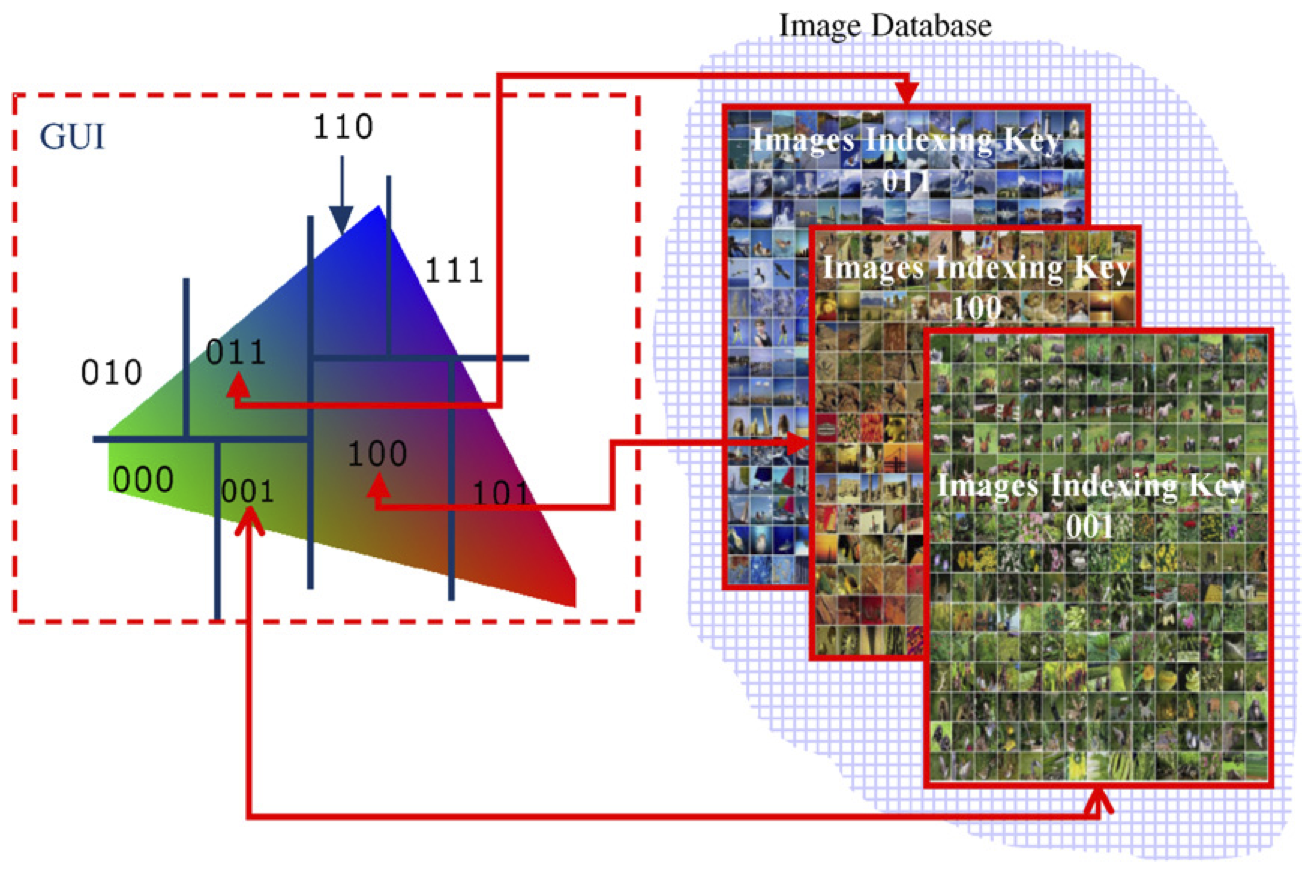
\includegraphics[width=0.6\columnwidth]{imgs-RelatedWork/Qiu-2007p1207.png}
	\caption[Chromacy diagram and color related images, from the work of Qiu et al.]{The chromacy diagram is split in parts and each image belongs to one of this parts. The diagram is part of the \ac{UI} and  when navigating through the diagram, only the images related to that part are shown.}
	\label{fig:qiu1}
\end{figure}

The system shows all the photos arranged by color, just as many others like it. The difference is the process in use. Instead of calculating distance vectors based on the histogram of each image, this approach classifies each image with a simple description, like an average of its colors, and arranges them by that value, on a color map (\fig{qiu1}). The process is much faster, but is also more error prone, specially on photos without a clear main color.

Their tests show they achieved good responsiveness and better results than using a file explorer.

% section Qiu (end)

\subsection{Does organization by similarity assist image browsing?} % (fold)
\label{sub:Rodden}
\begin{figure}[ht]
	\centering
		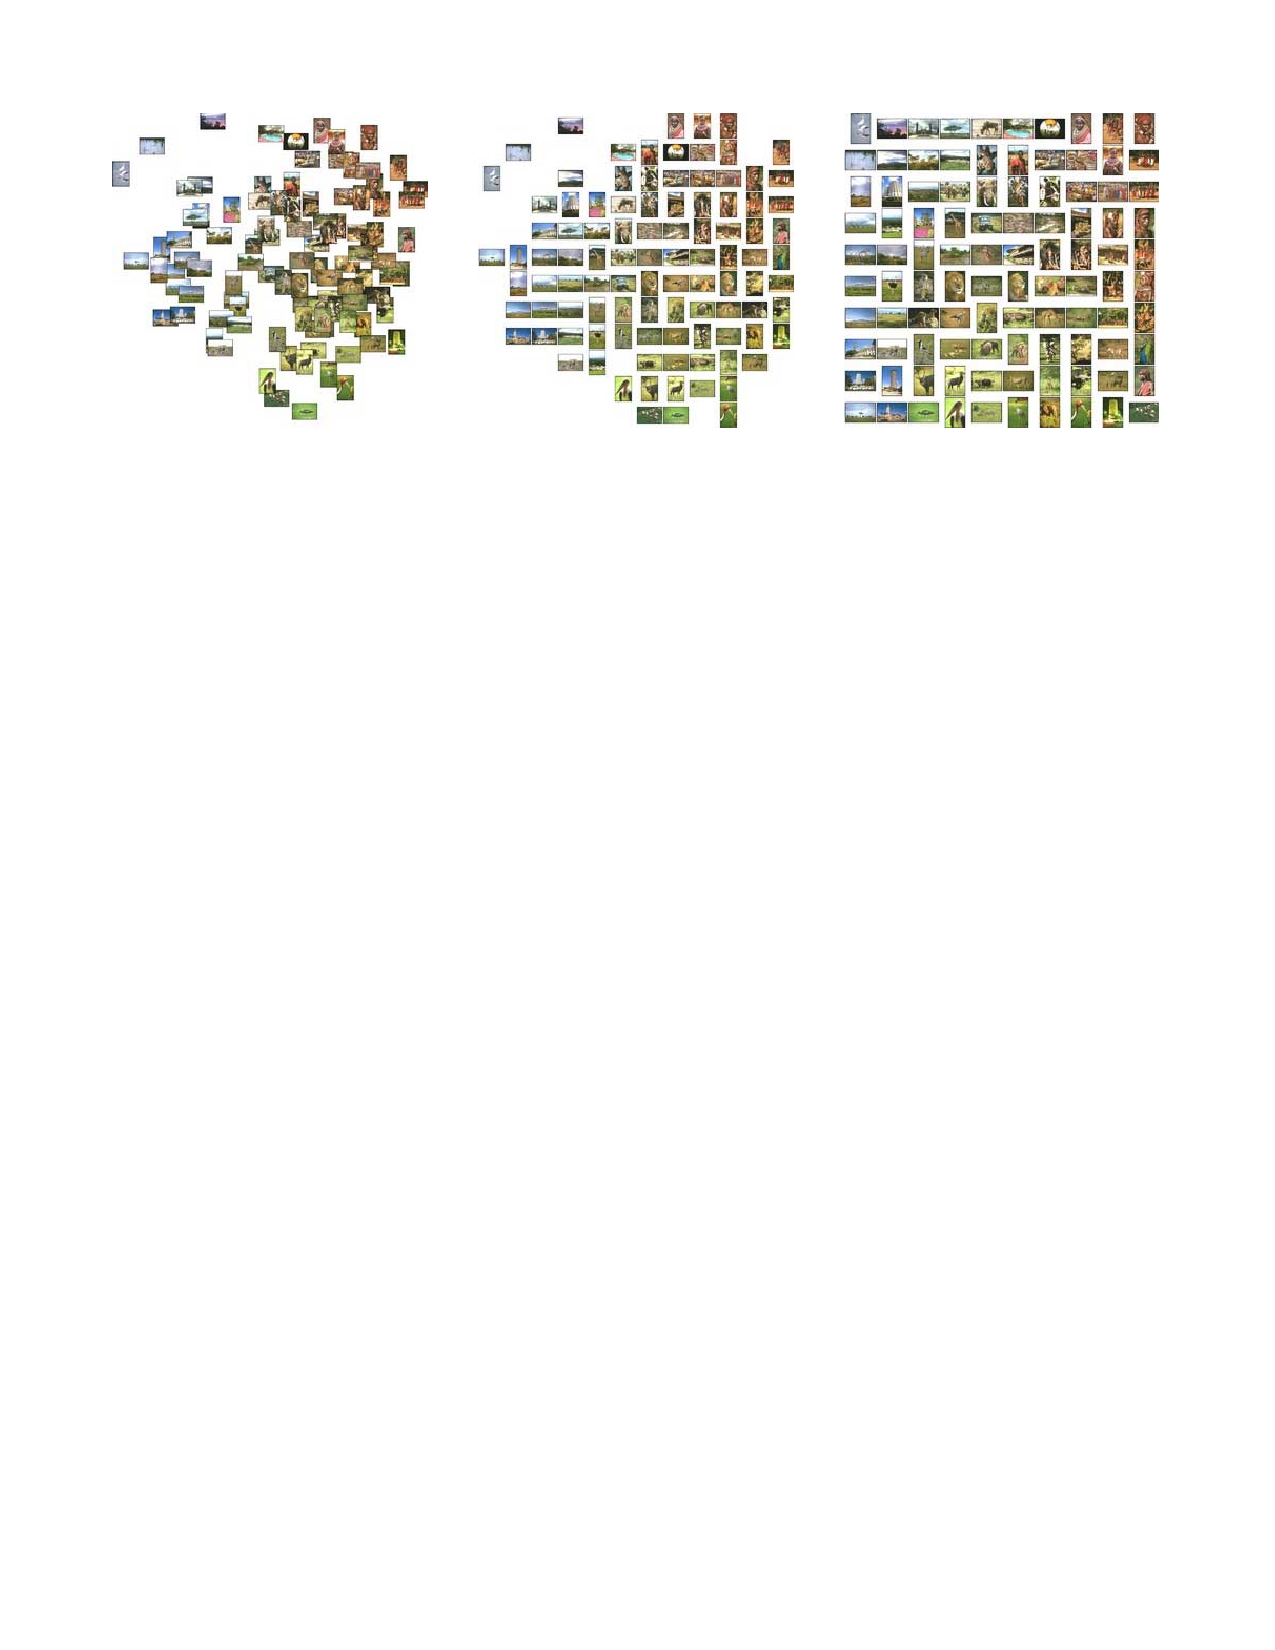
\includegraphics[width=\textwidth]{imgs-RelatedWork/Rodden1}
	\caption[Three arrangements of 100 images of Kenya, based on visual similarity, from the work of Rodden and Sinclar]{Three arrangements of 100 images of Kenya, based on visual similarity. On the left is the arrangement with overlap, in the middle a 12x12 grid (which removes the overlap while preserving some of the structure), and on the right a 10x10 grid (which maximises the thumbnail size).}
	\label{fig:Rodden1}
\end{figure}

The aim of this work by Rodden and Sinclar \cite{Rodden:2001p731} was to evaluate how photo organization by similarity (\fig{Rodden1}) could benefit a user looking for images. Some users tested an application that could show the same images both in a random and in an organized by similarity way. This organization by similarity was based on a rough description of the images, but it could be other descriptors.

The results differ if the user knows what he's looking for or not. In case he does, being able to filter only the relevant images makes it quick to find the ones that matter. This obviously depends on the quality of the labeling. Users reported that sometimes the similar images appear to merge.

In case the user doesn't know what he's looking for, the random approach might be helpful because the strong images usually contrast to their neighbors and thus appear to stand out.

For some people, having access to different arrangements of the same set of images is useful, although the source of the individual differences still needs to be determined.

% section Rodden (end)


\subsection{Browsing large collections of images through unconventional visualization techniques} % (fold)
\label{sub:Porta}

\begin{figure}[!htb]
  \begin{subfigmatrix}{2}
    \subfigure[Spot display]{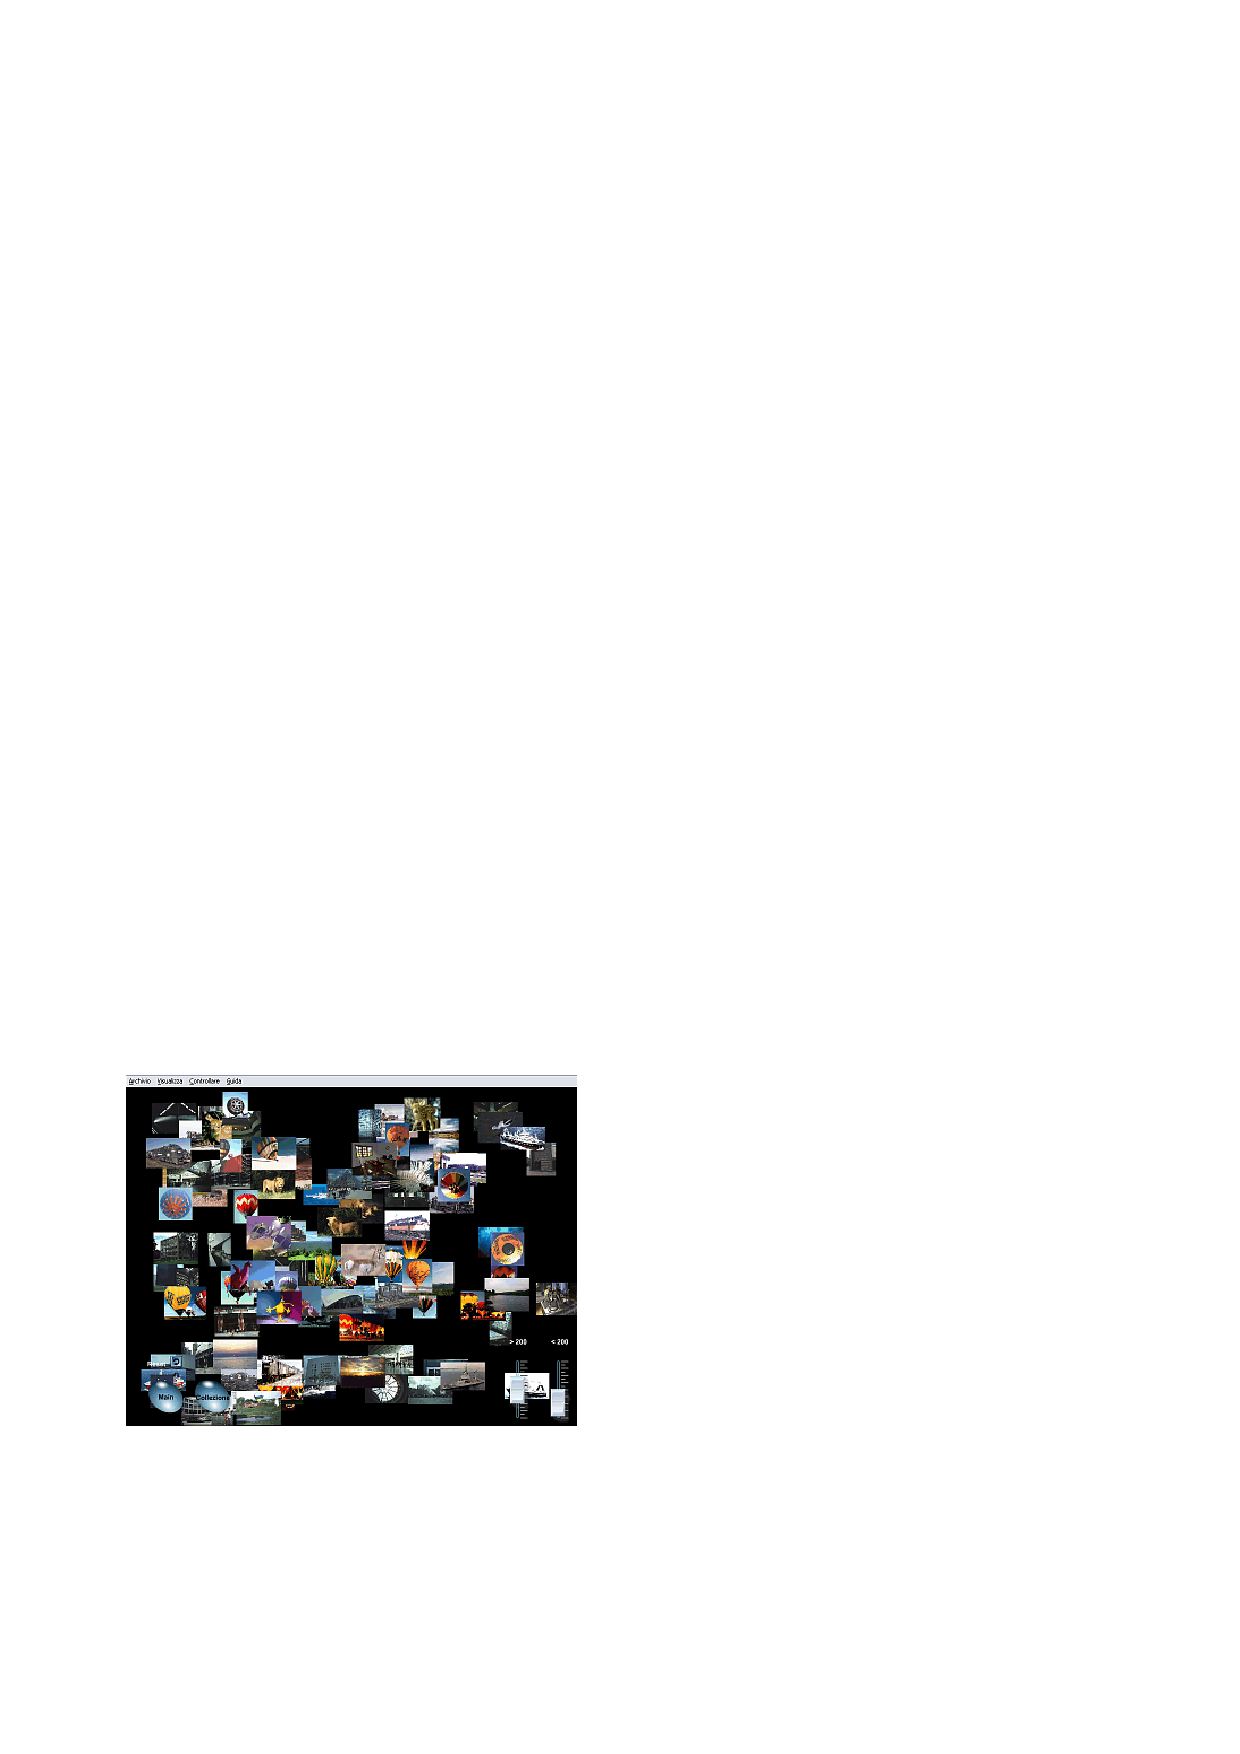
\includegraphics[width=0.49\linewidth]{imgs-RelatedWork/Porta-spot}\label{fig:porta-spot}}
    \subfigure[Shot display]{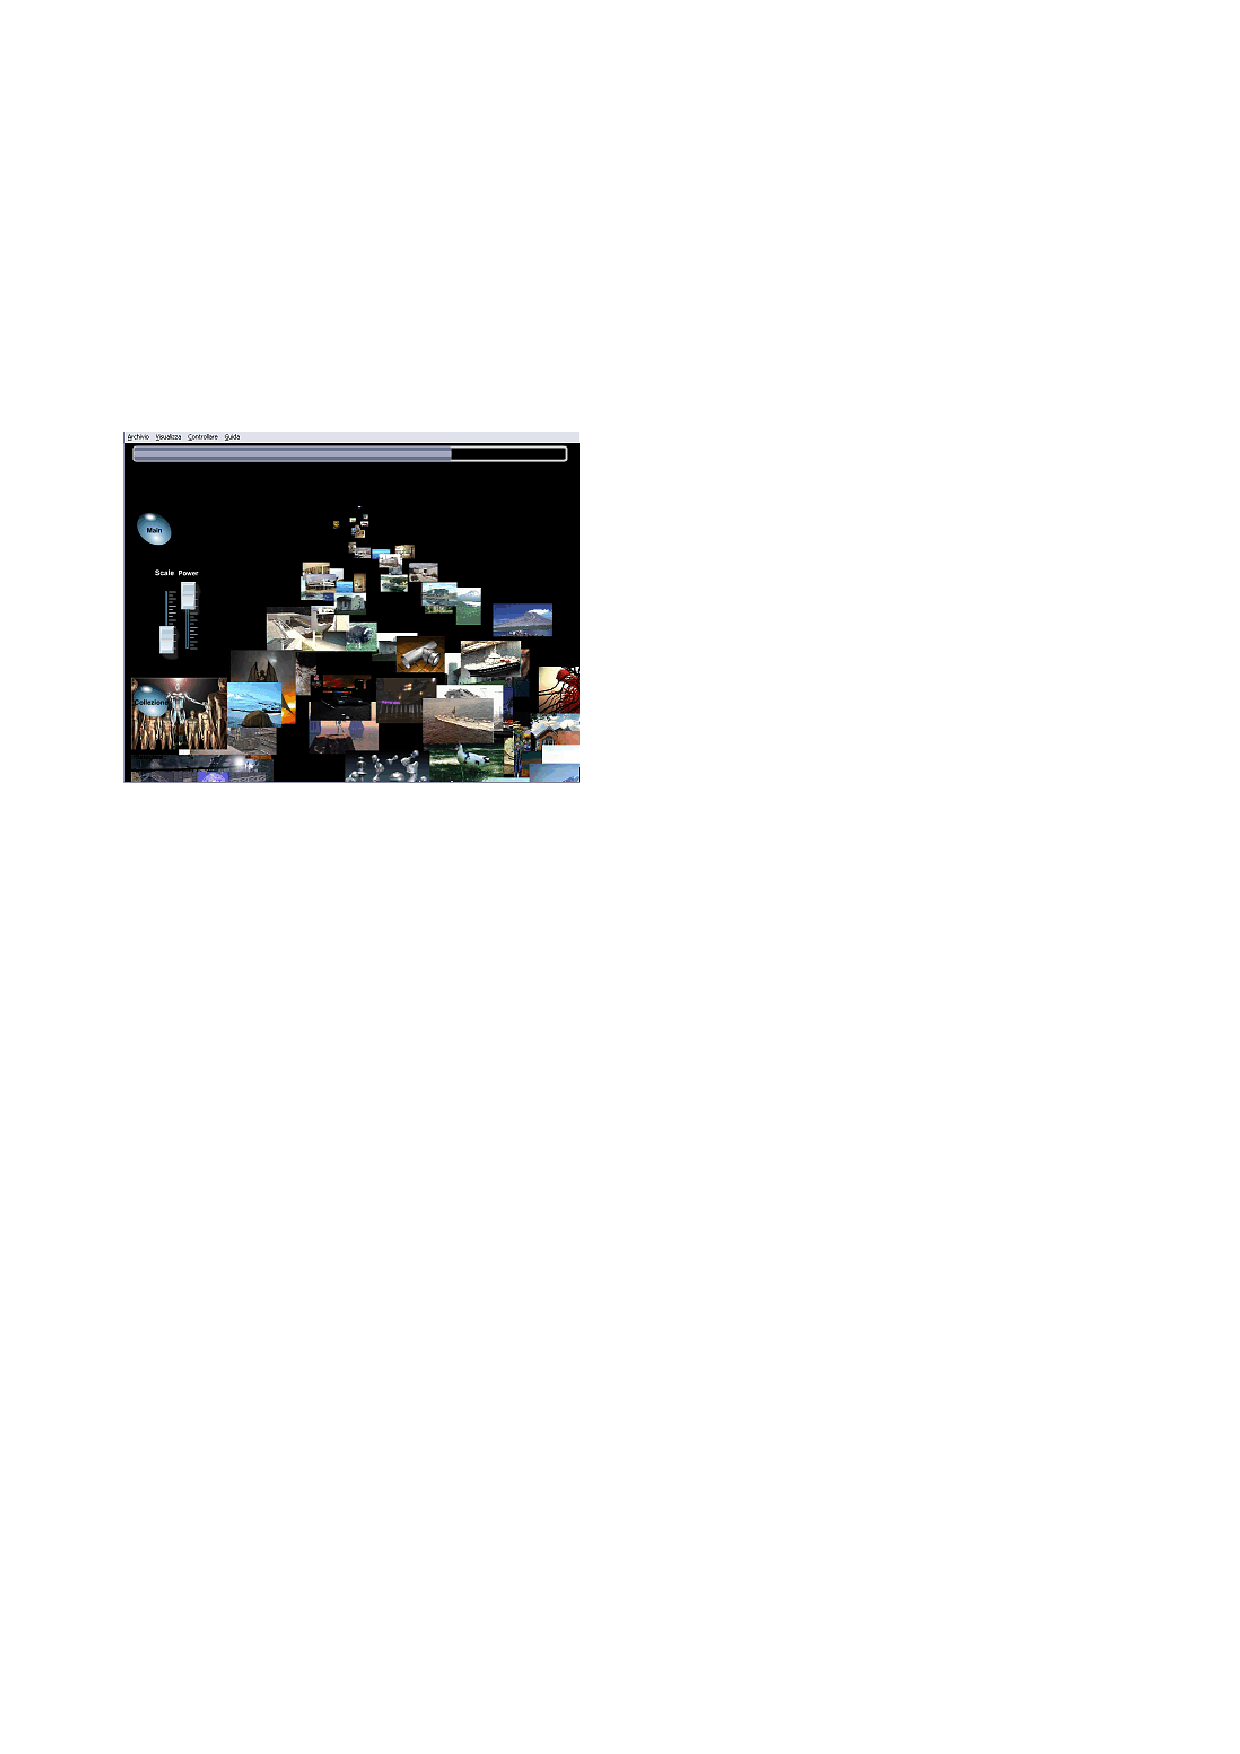
\includegraphics[width=0.49\linewidth]{imgs-RelatedWork/Porta-shot}\label{fig:porta-shot}}
  \end{subfigmatrix}
  \caption{The two better visualizations from Porta's work.}
  \label{fig:porta}
\end{figure}


Porta \cite{Porta:2006p416} describes a few visualization methods for large collections of images and tests them with users. The purpose is to find ways or metaphors that provide a good visualization experience in terms of time spent and quality of the visualization.

Some of the various techniques were the simple image grid view, a grid view with variable and independent height and width (EIB), a view that animates images like they were shot from a distance and get closer to the user called Shot (\fig{porta-shot}), a view where images quickly appear on random positions on screen named Spot (\fig{porta-spot}), and some other less commons like one that simulates a cylinder created with images (Cylinder), and others less relevant (Rotor, Tornado and Tornado of Planes).

The testing was based on the efficiency of users searching for specific images on a collection of a thousand photos. The Spot view was the best, followed the Shot, Cylinder finally the common grid view. The other views got scores near or below the grid view.

% section Porta (end)

\subsection{A comparison of static and moving presentation modes for image collections} % (fold)
\label{sub:Cooper}

This paper by Cooper et al. \cite{Cooper:2006p543} is not about large libraries, but about what kind of interfaces for image showing has greater success of user recognition and preference (\fig{Cooper1}).

With the help of eye-tracking techniques and user preference, the authors determined that static images are better than moving ones because makes them easier to recognize and avoid some user confusion.

\begin{figure}[ht]
	\centering
		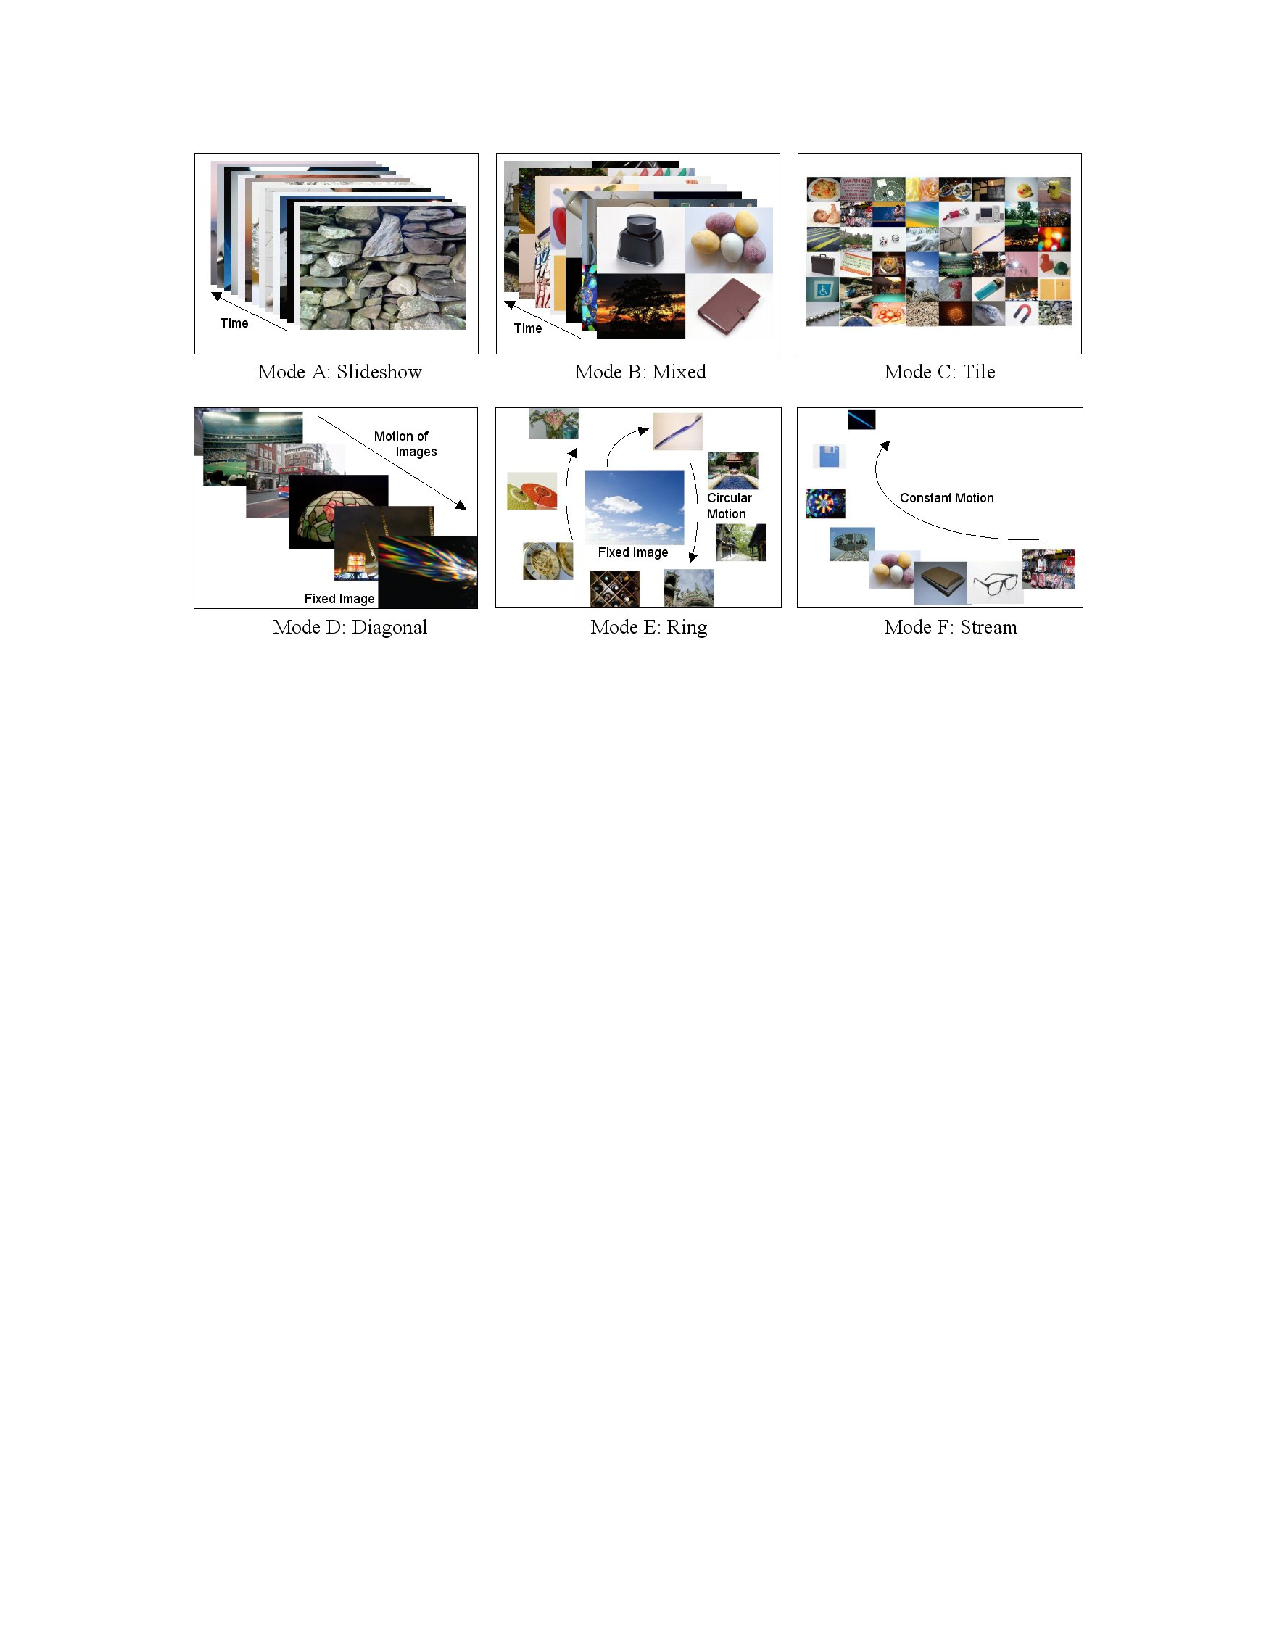
\includegraphics[width=\textwidth]{imgs-RelatedWork/Cooper1}
	\caption{The six rapid serial visual presentation modes used in the experiments}
	\label{fig:Cooper1}
\end{figure}
% section cooper (end)

\subsection{Organizing and browsing photos using different feature vectors and their evaluations} % (fold)
\label{sub:Strong}

Although it doesn't mention why, Strong \cite{Strong:2009p413} focuses on the better experience provided by color organization of a large image collection (\fig{Strong1}).

A \ac{SOM} is used to display the images on the screen featuring zooming, panning and sorting capabilities. The work is then based around the various methods used to determine the images' similarity.

Simpler methods are based on color histograms, which aren't affected by rotations or scales but, by not having spacial information on colors, allows very different images be closer together.

Other methods rely on gradients which contain spatial information and, therefore, are sensitive to image contents, but not color.
In general, the best methods were found to be the hybrid ones, where both color histograms and gradients are used to classify the images.
No user testing is made in this project, neither is the speed of image categorization referred about the methods used.

\begin{figure}[ht]
	\centering
		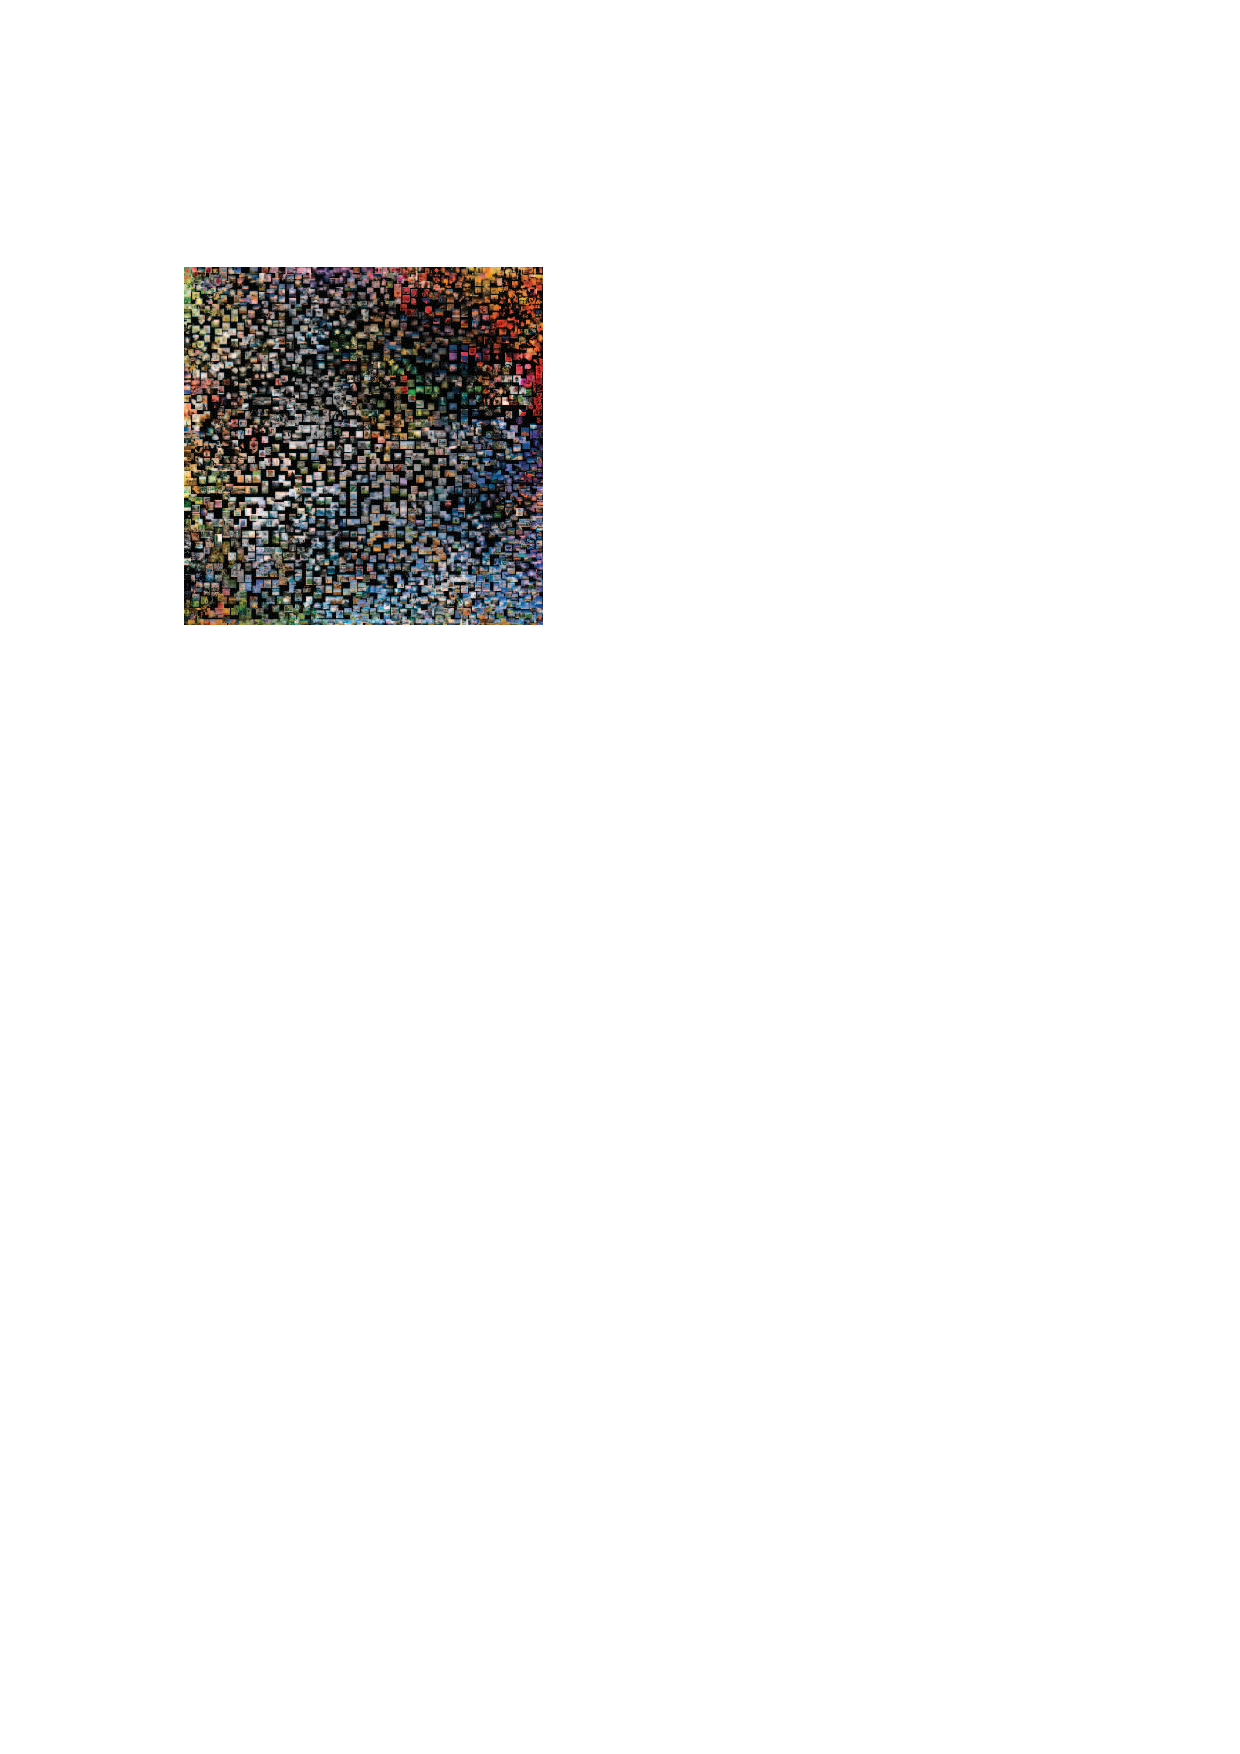
\includegraphics[scale=1]{imgs-RelatedWork/Strong1}
	\caption{The result obtained for organizing 2200+ photos using color autocorrelogram feature vector, using Strong's work \cite{Strong:2009p413}.}
	\label{fig:Strong1}
\end{figure}

% section strong (end)

\newpage
\subsection{An evaluation of color-spatial retrieval techniques for large image databases} % (fold)
\label{sub:Tan}
% não tem imagens

Tan et al. \cite{Tan:2001p850} present an evaluation of three color-spatial image retrieval techniques.

The signature-based technique creates a signature for each image, based on the most frequent colors, according to a threshold, of each subdivision, or bin, of that image. The comparison between images is made by comparing the main colors present on each bin. It is possible to assign more weight to specific bins according to the user's interest.

The partition-based approach is also based on bins, each having it's own color histogram. The similarity between images is given by the distance of the histograms of the corresponding bins.

The cluster-based method bases on the fact that humans focus on large patches (clusters) of the same color and, therefore, two images will appear similar if both have similar colored clusters on at roughly the same location. This method extracts the larger clusters and their color from each image. The similarity is calculated by the amount of overlap between clusters.

This techniques were tested with a collection of 12,000 images and, besides the color information, the brightness was also analyzed for increased performance. The authors conclude the signature method was generally better on both effectiveness and efficiency.

% section tan (end)

\subsection{Automatic organization for digital photographs with geographic coordinates} % (fold)
\label{sub:Naaman}

In this paper, by Naaman et al. \cite{Naaman:2004p1802}, is described a system that organizes digital photographs accordingly to location and date embedded on the metadata.

The objective was trying to mimmic the way people think about their collections. Photos are usually bursts separated by some time. Based on this and on the different places, events can be created to agglomerate photos from the same bursts. Location naming is done by calculating the most relevant places, like parks or cities, and then mixing the more precise locations with the more important neighbor cities to create a relevant and identifiable name. This was specially important since this work didn't involve showing any maps, but only the location names and events.

The authors showed good results and, nowadays, some common applications use similar features although including maps.
% section naaman (end)

\subsection{Similarity pyramids for browsing and organization of large image databases} % (fold)
\label{sub:Chen}

Chen et al. \cite{Chen:1998p2344} present a method for designing a hierarchical browsing environment called a similarity pyramid. The similarity pyramid groups similar images together while allowing users to view the database at varying levels of resolution. Each level is organized such that similar images are in close proximity on a two-dimensional grid (\fig{Chen1}). Images are first organized into a binary tree through agglomerative clustering based on color, edge and texture similarities. The binary tree is transformed into a quadtree, a tree in which each node has four children instead of only two.

\begin{figure}[ht]
	\centering
		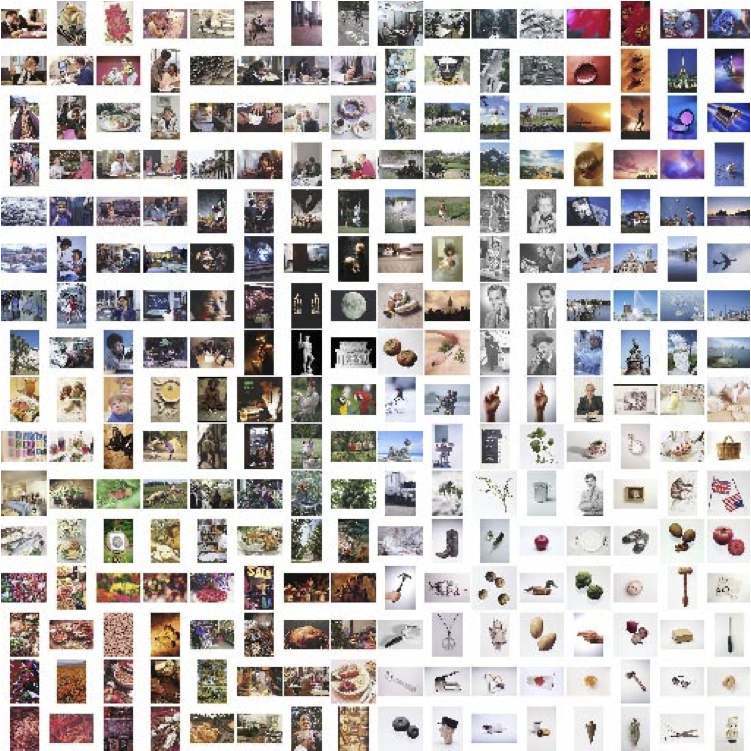
\includegraphics[scale=0.8]{imgs-RelatedWork/Chen-1998p2344.png}
	\caption{Images organized with \cite{Chen:1998p2344}. Images with similar color and texture are spatially adjacent.}
	\label{fig:Chen1}
\end{figure}

The similarity pyramid is best constructed using agglomerative (bottom-up) clustering methods, and a fast-sparse clustering method is presented which dramatically reduces both memory and computation over conventional methods. This method is based on the flexible agglomerative clustering algorithm, but using only a sparse proximity matrix and exploiting the author's approximate branch and bound search algorithm.

The authors found that the method for mapping the clustering to a pyramid can make a substantial difference in the quality of organization. Finally, a dispersion metric for objectively measuring pyramid organization was proposed, and found that it correlated well with the author's subjective evaluations of pyramid organization.

% section Chen (end)


\subsection{NN\super{k} networks for content-based image retrieval} % (fold)
\label{sub:Heesch}

Heesch \cite{Heesch:2004p2675} describes a different interaction technique for content based search in large image collections. Each image is a vertex in a graph and arcs are established between images if there exists at least one combination of features for which one image is retrieved as the nearest neighbor of the other. Each arc is weighted by the proportion of feature combinations for which the nearest neighbor relationship holds. By integrating the retrieval results over several feature combinations, the resulting network helps expose the semantic richness of images.

The interface reflects the vertexes and respective arcs, allowing to browse between the related images (\fig{heesch1}) in the network.

\begin{figure}[ht]
	\centering
		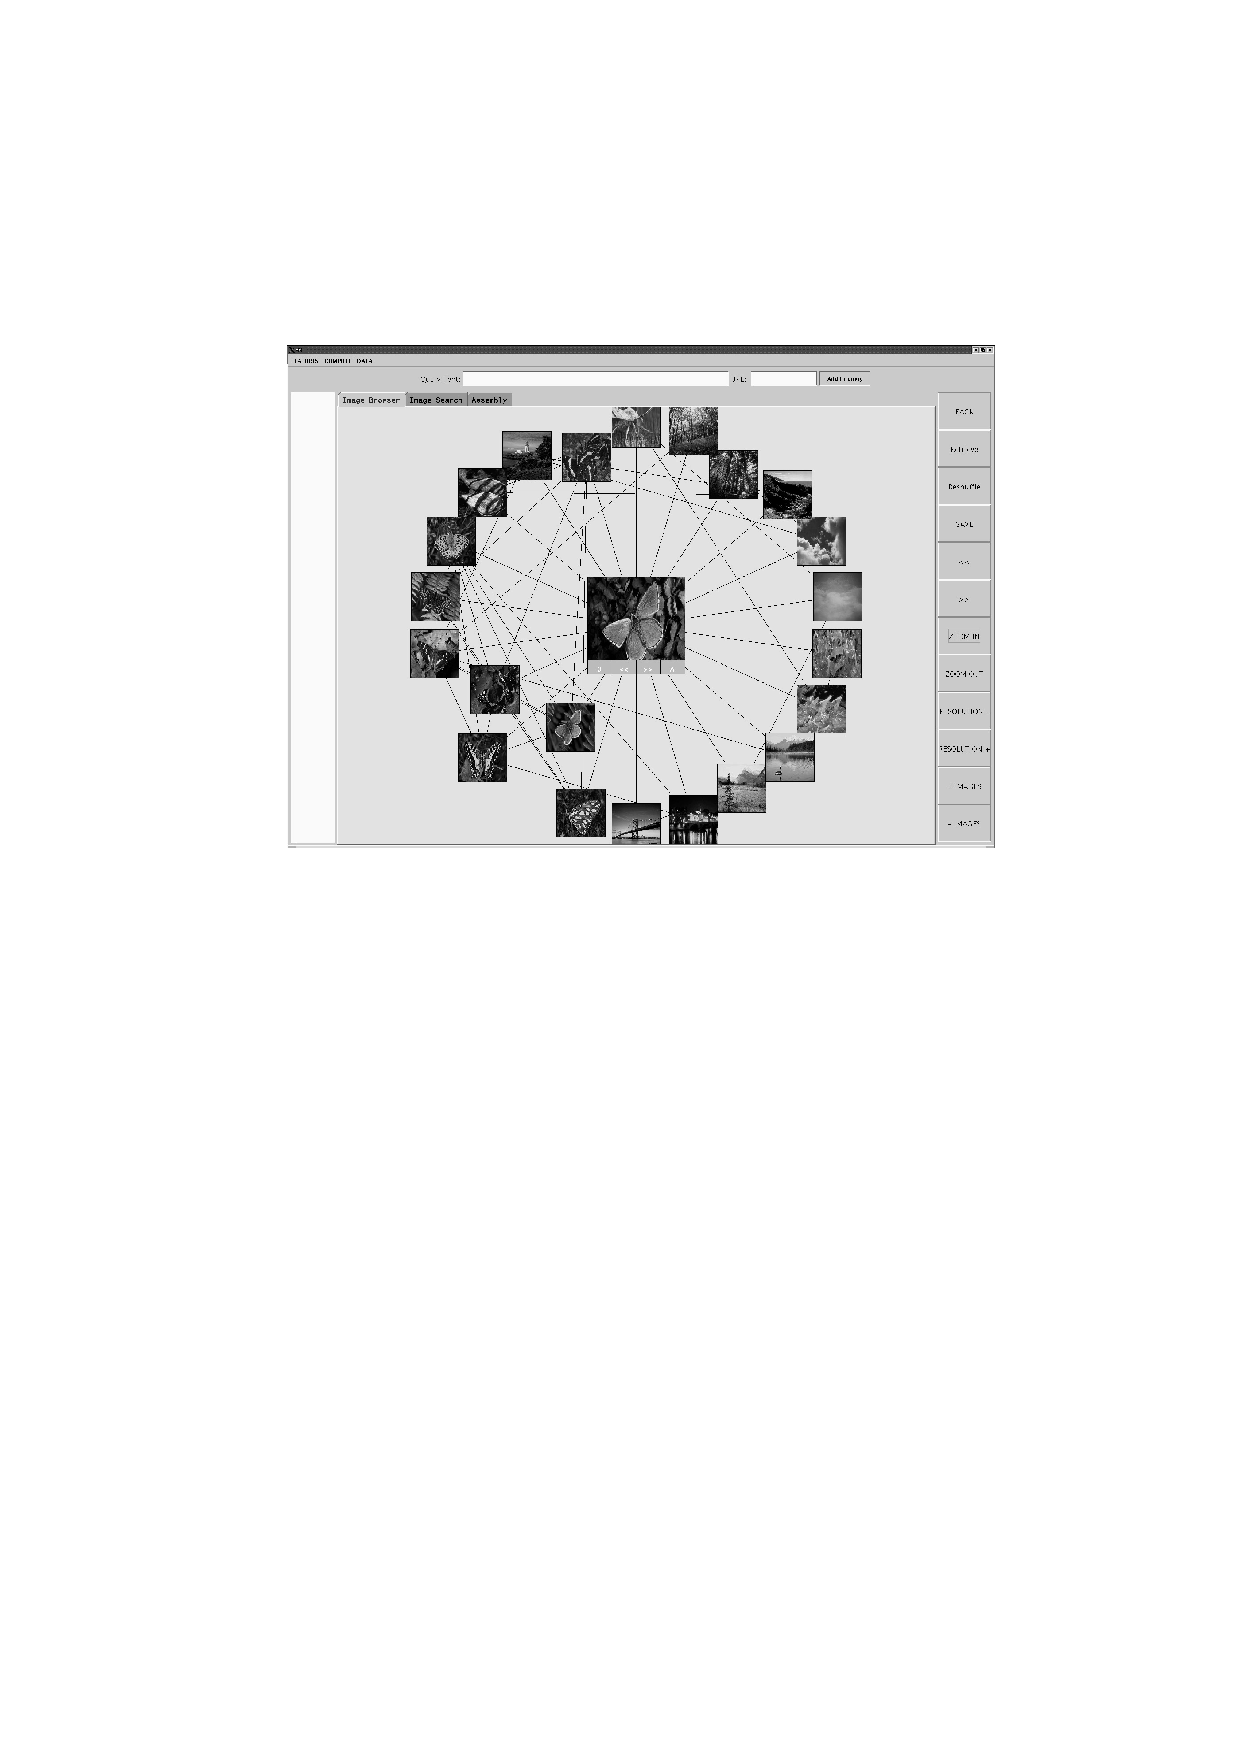
\includegraphics[scale=1]{imgs-RelatedWork/Heesch-2004p2675}
	\caption{Local network around the chosen butterfly image depicted in the middle.}
	\label{fig:heesch1}
\end{figure}

Seven low-level features are used for the classification of the images. HSV Global color Histograms maps the images by color, saturation and brightness; color Structure Descriptor maps the distribution of colors by dividing each image in 64 windows, the color space in 184 bins and associating color bins with image windows; Thumbnail feature compares identical images by saving the grey value of each pixel from a scaled down version of the image; Convolution filters discovers very selective features by reapplying 25 filters three times; Variance feature calculates standard deviations within a sliding window; Uniformity Feature is another statistical feature, calculating the grey level of an image split in 64 parts; Bag of words is the last feature and weights words associated to each image.

Tests showed great results when using a mix of search, relevance feedback and browsing, and even browsing by itself was considerably better than other, more restrictive, approaches.

The technique helps avoid the problem of image polysemy by showing all gathered meanings of the images to the user.
The feature network is pre-computed, allowing for quick realtime browsing. The authors claim it took 50 hours to process 32000 images, but made no reference to the possibility adding images to the collection, after the computation.

% section heesch:2004p2675 (end)

\subsection{Phorigami: A Photo browser based on meta-categorization and origami visualization} % (fold)
\label{sub:Hsu}

Hsu et al. \cite{Hsu:2009p2696} try to ease the browsing problem by analyzing the collections and identifying groups of related pictures. Each type of group is visualized in a specific way, inspired by the Origami art.

Groups of similar or related photos were manually classified based on camera movement and subject movement, creating different types of groups static view where both camera and subject are fixed and is presented as a panorama; multi-view where the subject is fixed, but the camera is moving and is shown as a presentation; if the subject is moving, the photos are categorized as motion capture and can be shown as an animated photo (fixed camera) or a presentation (moving camera); finally group photos, where different groups of people are photographed, are shown as a folding presentation.

This covers various cases where the photographer takes a few similar photos of the same subject because it's either a panorama, various angles or just to be sure the photo was well captured. 

The interface implements the different presentation types as different metaphors, easy for the user to understand, like a folded paper on a wide panorama that can be expanded (\fig{hsu1}). Although some of them appear to be a little hard to distinguish in its compressed form, it shouldn't be difficult to make it clearer. Other possible problem is the use of different touch interactions for each presentation type that might confuse users on what gesture should they use.

\begin{figure}[ht]
	\centering
		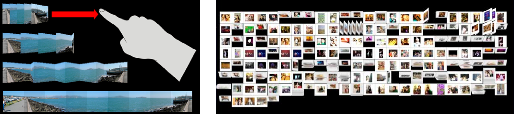
\includegraphics[width=\textwidth]{imgs-RelatedWork/hsu.png}
	\caption[Hsu's work of grouping together related images]{On the left, an example of an interaction on a group of photos that makes a panorama. On the right, a visualization on 537 photos with some groups.}
	\label{fig:hsu1}
\end{figure}


% section hsu:2009p2696 (end)

\subsection{A next generation browsing environment for large image repositories} % (fold)
\label{sub:Schaefer}

\begin{figure}[ht]
	\centering
		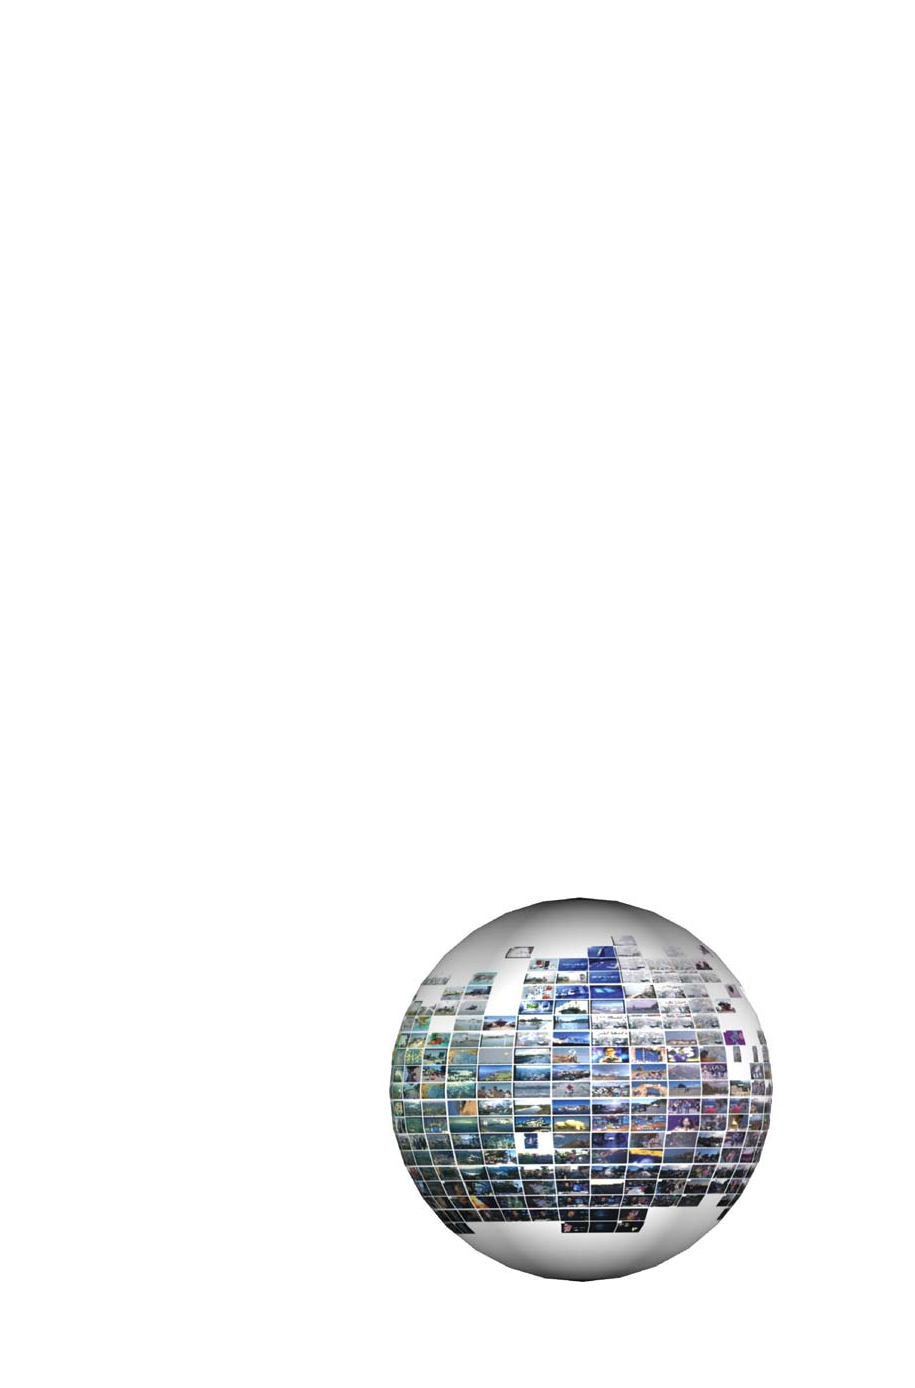
\includegraphics[scale=1]{imgs-RelatedWork/shaefer1.pdf}
	\caption{Hue sphere of a dataset, from Schaefer's work.}
	\label{fig:schaefer1}
\end{figure}

Schaefer \cite{Schaefer:2010p1871} tries to take similarity based organization of images from the 2D space to a 3D sphere, which allows interaction from the users. Rotating the sphere reveals images with different colors while tilting it reveals brighter or darker images.

Large image collections are handled through a hierarchical approach that brings up similar, previously hidden, images when zooming in on an area.

The description of the color is retrieved by calculating the image's median color for it's efficiency over other methods like histograms. This two features are directly mapped onto the sphere's coordinates and the entire structure is pre-calculated so browsing can be performed in real-time. Image overlapping is also avoided (\fig{schaefer1}).

The work was tested on a 4500 image collection with no evaluation as to its performance and a weak and subjective user testing.


% section schaefer:2010p1871 (end)

\subsection{Flexible access to photo libraries via time place, tags, and visual features} % (fold)
\label{sub:Girgensohn}
\begin{figure}[ht]
	\centering
		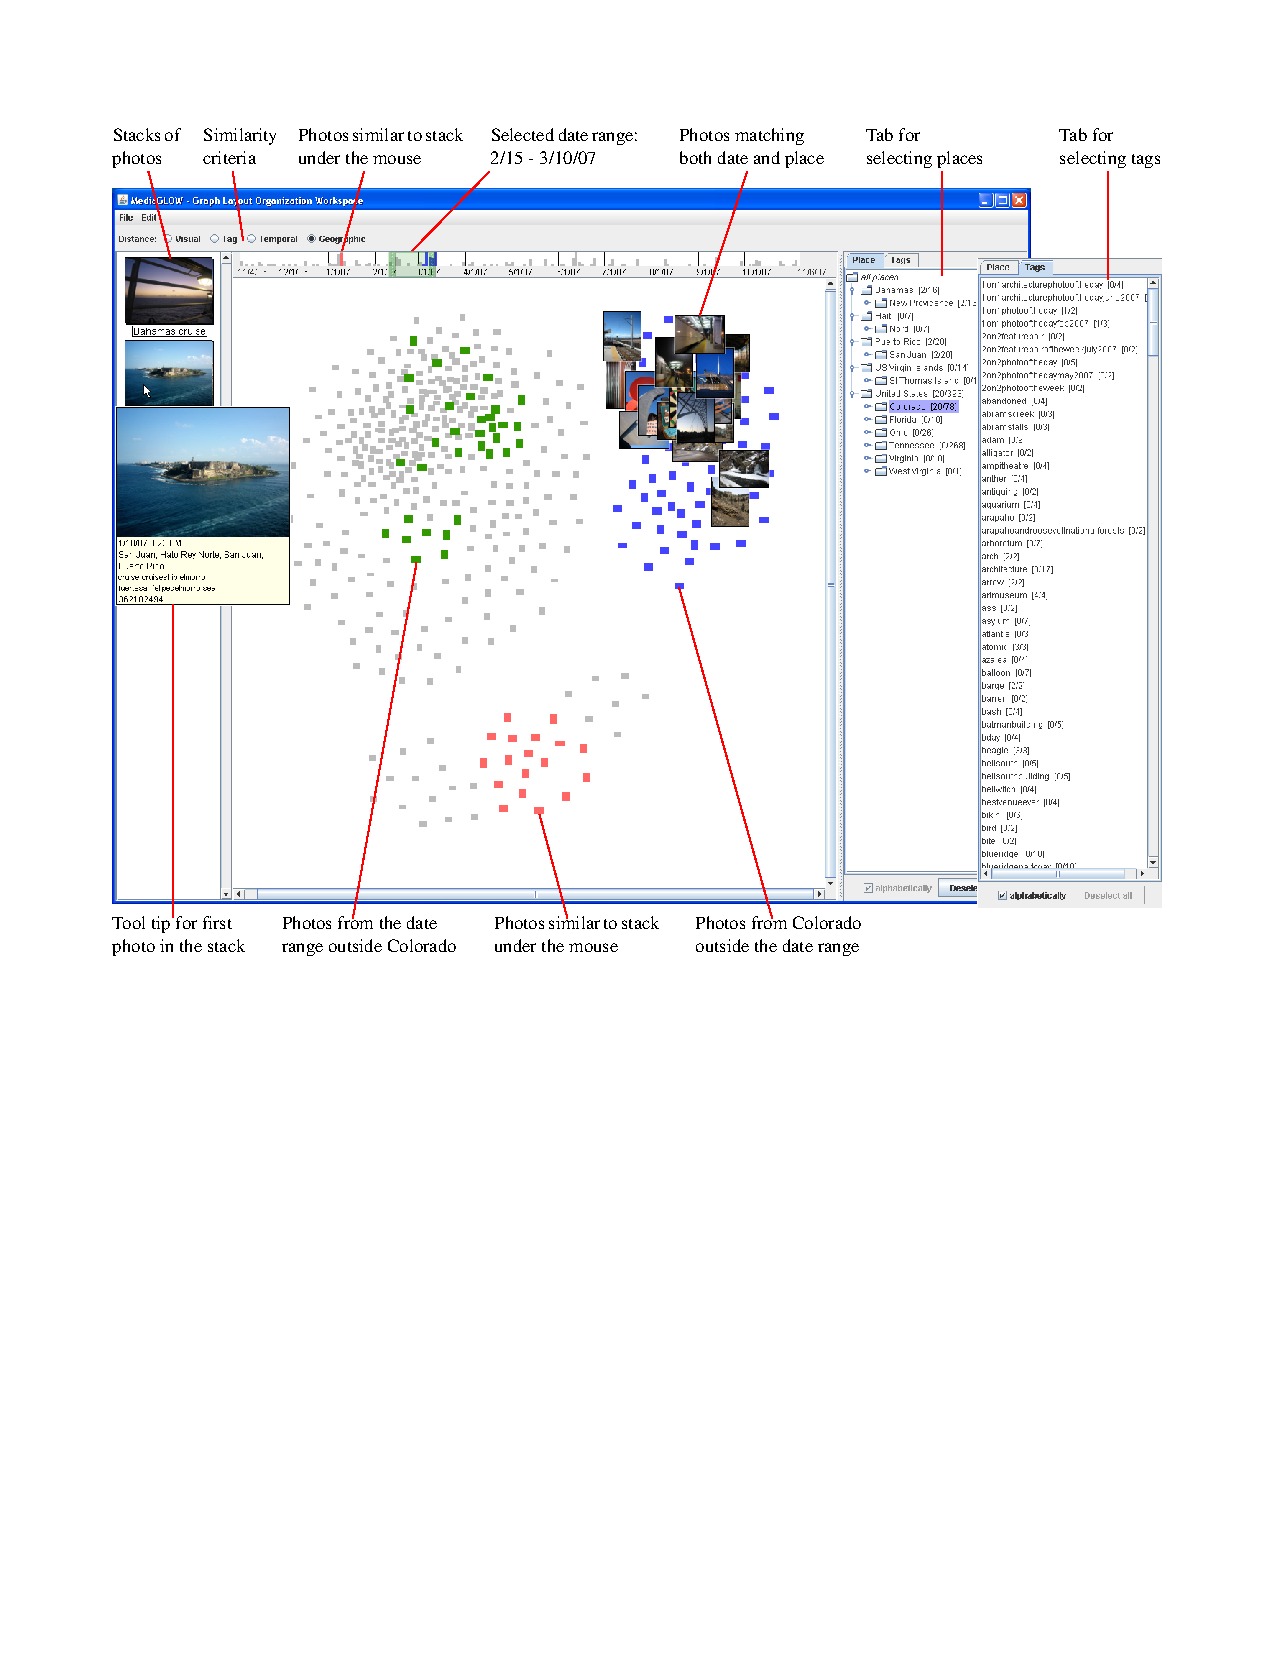
\includegraphics[width=\textwidth]{imgs-RelatedWork/Girgensohn1.pdf}
	\caption{Photos grouped by geographic similarity and filtered by date and place.}
	\label{fig:girgensohn}
\end{figure}

MediaGLOW by Girgensohn et al. \cite{Girgensohn:2010} is the application discussed in this paper. It's a \ac{CBIR} system with multiple ways to filter and sort the image collection.

The interface allows selecting a range of dates, places and tags at any time to filter the collection and the display will show the photos that match the filters, alongside indications of the existence of photos that match some of the filters. This display can then be arranged by four similarity criteria: temporal (by photo creation time), geographic (distances between places), tags (photos with similar tags are shown closer together) and visual (\fig{girgensohn}).

The time is selected using a timeline on the top of the screen while tags and places are shown on the right side sorted alphabetically, by frequency of, in case of places, as a tree. Multiple selections are allowed to show more photos.

The photo display is graph based, allowing for overlapped images. Various metaphors were developed to ease the navigation of the collection. Zooming is allowed and changes both thumbnail positions and size for better experience, allowing the photos to spread away from each other, but also increasing the size so the user can have a better look at them. The authors think that bigger thumbnails and a correct grouping of related photos is more important than spreading them to avoid the overlapping problem.

Color coding is used throughout the interface to help the user understand better what is being selected. For instance, on the timeline blue and grey are used to distinguish photos that match or not the selected location/tag. On the photo display, besides the photos that are actually shown are colored blocks: blue for photos that match location only, green for time only and grey for those that didn't match anything.

Detailed user testing was performed and the importance of the multiple ways to organize and search the collections was emphasized since many systems are designed to have a single form of access. Some users also pointed the importance of being able to have a non overlapping view of the photos for part of the task.

Each view was found to have different levels of usage, the geographic being the most used and temporal the least, since it's very similar to the timeline. Visual similarity was less used than expected, even on collections where it was relevant. 




\subsection{PhotoMesa: a zoomable image browser using quantum treemaps and bubblemaps}
\label{sub:PhotoMesa}

This work presents PhotoMesa by B. B. Bederson \cite{Bederson:2001:PZI:502348.502359}, an application that supports browsing sets of images in a zoomable environment. It also supports clustering by metadata, not requiring previous work from the user. Users can choose directories of images and they are all displayed in a space-filling manner \fig{photomesa}. Images are displayed in groups, from the directories they origin from and users can smoothly zoom in to a group and then to a single image. It generates multiple-resolution thumbnails for maintaing a good performance. Keyboard keys are also used to navigate the canvas. The groups display their name and have different background colors for a better distinction. It also supports drag and drop of images to other applications. Text search is possible as well as selecting a group on a list.

\begin{figure}[ht!]
	\centering
		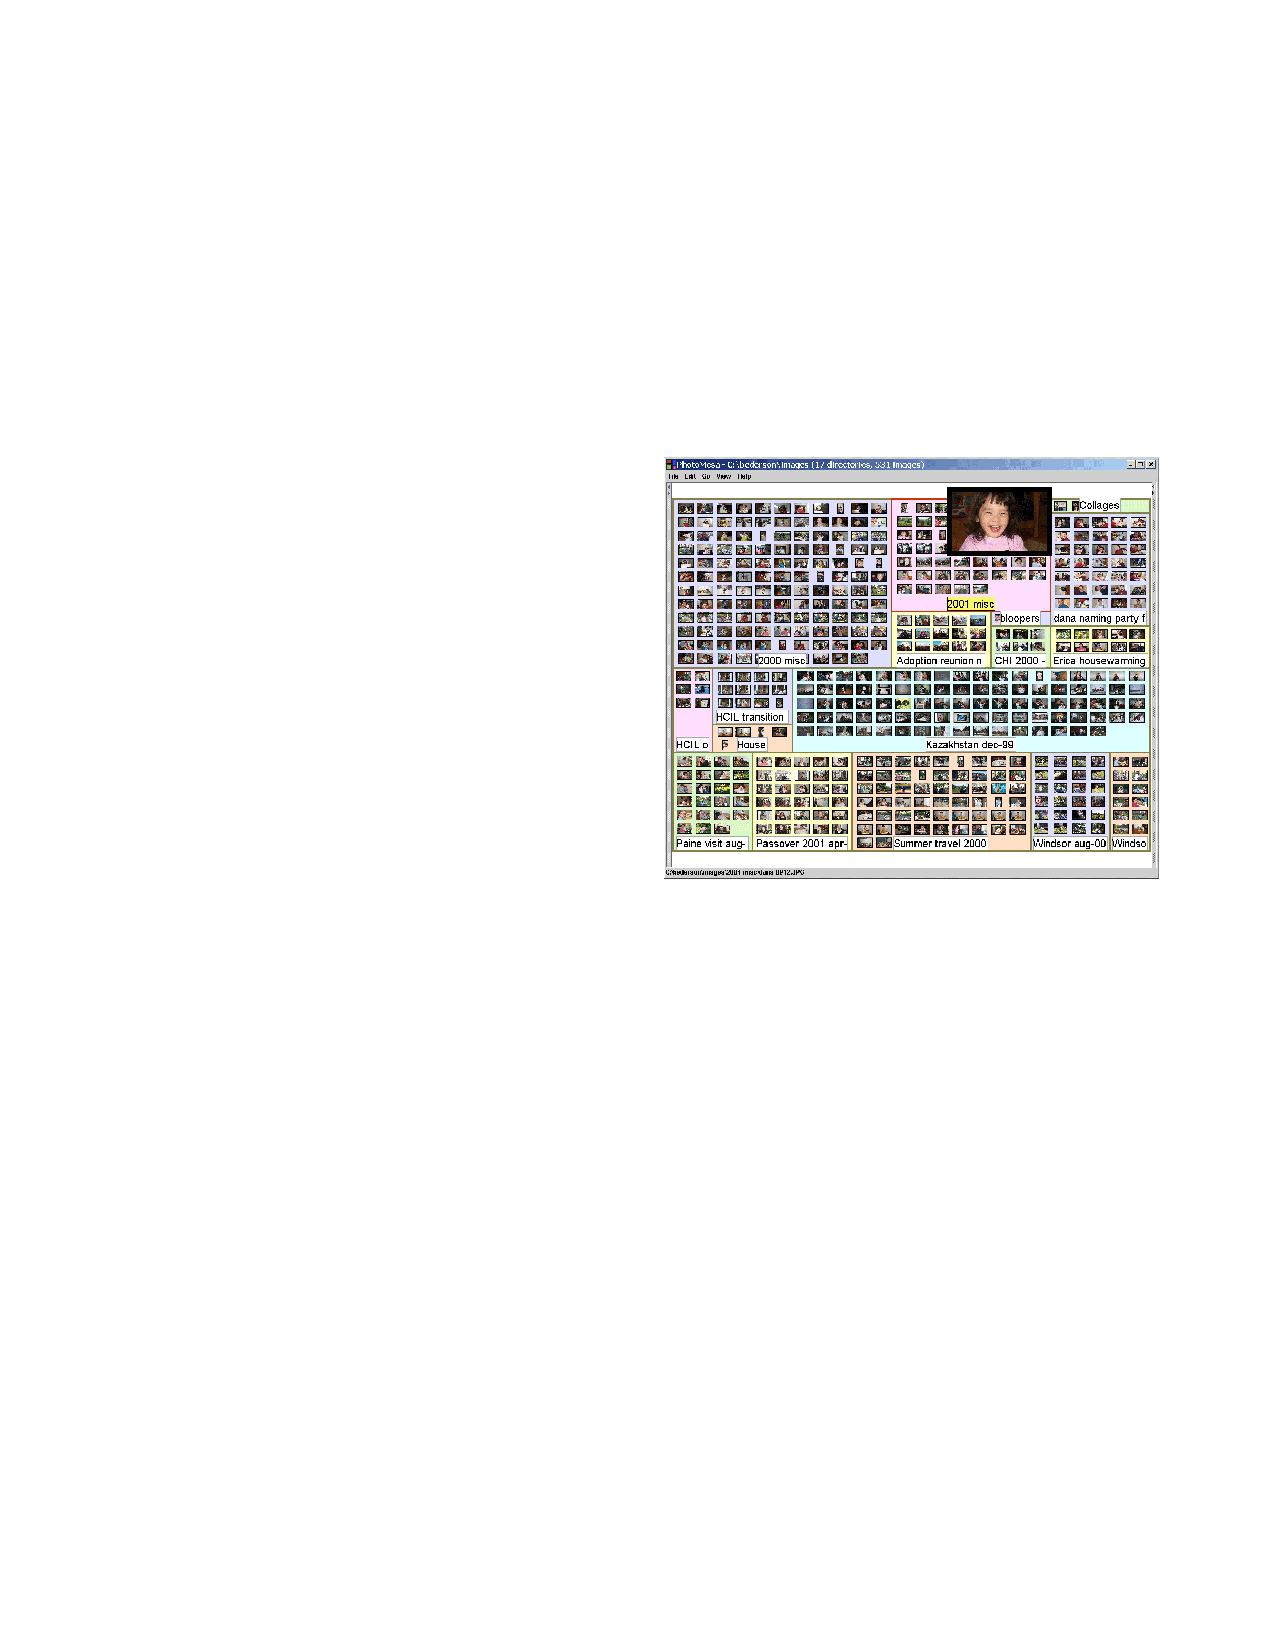
\includegraphics[width=0.90\textwidth]{imgs-RelatedWork/PhotoMesa.pdf}
	\caption{PhotoMesa with over 500 images in 17 groups.}
	\label{fig:photomesa}
\end{figure}

PhotoMesa implements two algorithms for space filling, one is Quantum Treemaps by the author, a variation of the Ordered Treemap  that is aware of the constraints imposed by the use of images, like grid alignment and common size, and Bubble Maps which is designed to have the least wasted space possible.

This work brings very interesting ideas to the table, but it has a somewhat limited reach, with only referring to ``over 500 images'' on the application and by only taking simple metadata, like the path and modification date of images.




% section girgensohn:2010 (end)

\section{Discussion} % (fold)
\label{sub:discussion}


Currently there are a lot of approaches to image organization and each has its own differences as demonstrated on Table \ref{tab:brows-meth}. Our survey went by multiple works and revealed various methods for extracting the features from each image, multiple visualization methods from grids to flying images.


\begin{table}[ht]
 \begin{tabular}{| m{2.7cm} |>{\centering}m{2.3cm}|c|c|c|>{\centering}m{2.1cm}|>{\centering}m{2.3cm}|r|}
  \hline
\multirow{2}{*}{\textbf{Work}} & \multicolumn{4}{c|}{\textbf{Organization}} & \multirow{2}{*}{\textbf{Visualization}} & \multirow{2}{*}{\textbf{Focus}} & \multirow{2}{*}{\textbf{Size}} \\
\cline{2-5}
	& \textbf{features} & \textbf{date} & \textbf{gps} & \textbf{tags} & & & \\

\hline 1.	Qiu \cite{Qiu:2007p1207}	& simple color measures 			& --- & --- & --- & Grid 			   & Simplicity and Efficiency 			& 60,000	\\
\hline 2.	Rodden \cite{Rodden:2001p731}	& --- 								& --- & --- & \cm & Grid 			   & Similarity usefulness	 			& 	 100	\\
\hline 3.	Porta \cite{Porta:2006p416}	& --- 								& --- & --- & --- & Spot (and others)  & Unconventional visualizations		& 	 400	\\
\hline 4.	Cooper \cite{Cooper:2006p543}	& --- 								& --- & --- & --- & Static and animated& Usefulness of animations 			& 	 ---	\\
\hline 5.	Strong \cite{Strong:2009p413}	& color histograms and gradients 	& --- & --- & --- & \ac{SOM} 		   & Evaluation of different features	&  2,200 	\\
\hline 6.	Tan	\cite{Tan:2001p850}		& color histograms of subdivisions & --- & --- & --- & --- 			   & Evaluation of different features 	& 12,000 	\\
\hline 7.	Naaman	\cite{Naaman:2004p1802}	& --- 								& \cm & \cm & --- & --- 			   & Organization based on events 		& 	   N/A	\\
\hline 8.	Chen	\cite{Chen:1998p2344}	& colors, edges and textures 		& --- & --- & --- & --- 			   & Efficient fast-sparce clustering 	& 10,000 	\\
\hline 9.	Heesch	\cite{Heesch:2004p2675} & six different features 			& --- & --- & \cm & Radial 			   & Complex similarity network 		& 32,000 	\\
\hline 10.	Phorigami, Hsu	\cite{Hsu:2009p2696}	& --- 								& --- & --- & --- & Grid with groups   & Interaction on grupped photos 		&  1,333 	\\
\hline 11.	Schaefer \cite{Schaefer:2010p1871} & color histograms of subdivisions & --- & --- & --- & 3D Sphere		   & 3D mapping and interaction 		&  4,500 	\\
\hline 12.	MediaGLOW, Girgensohn \cite{Girgensohn:2010}	& --- 								& \cm & \cm & \cm & Overlapped graph   & Having the best way to find photos &    450	\\
\hline 13. PhotoMesa, Bederson \cite{Bederson:2001:PZI:502348.502359} & --- & \cm & --- & \cm & Q. Treemap / Bubblemap & Zoomable browser & 500	\\
\hline
 \end{tabular}
\caption{Different browsing methods}
\label{tab:brows-meth}
\end{table}

One of the main problems is obtaining useful information from low level feature extraction of the image contents. Some try to get the most out of each image, with a variety of complex and time consuming procedures, e.g., a variety of methods based on color histograms \cite{Strong:2009p413,Tan:2001p850,Chen:1998p2344,Schaefer:2010p1871} or even more detailed ones with textures and convolution filters \cite{Heesch:2004p2675}. Others try to focus on avoiding the complex computations by only getting simple, but somewhat useful information \cite{Qiu:2007p1207}. To contrast with these methods, Girgensohn's work \cite{Girgensohn:2010} has found that users prefer other ways to filter the collection, like tags, dates and locations. Low level features are still used, but they have to be kept to understandable and useful options.

Date and location are simple similarity measures and can be used to group the collections by events and locations like Naaman did on this work \cite{Naaman:2004p1802}. Current mainstream software like Apple's iPhoto\footnote{http://www.apple.com/iphoto} or Google's Picasa\footnote{http://picasa.google.com} are already doing it in a semi-automatic way.

Textual metadata like tags and descriptions are also widely used both on our survey \cite{Rodden:2001p731,Girgensohn:2010,Heesch:2004p2675,Bederson:2001:PZI:502348.502359} and on all mainstream software. The problem with tags and descriptions is that people usually don't assign them to their photos, but that's not a problem we're interested here.

The visualization is the field with most variations and experimentations, like Porta's work \cite{Porta:2006p416} where multiple options were tested, but only a couple of the most simple were considered useful. The 3D Sphere \cite{Schaefer:2010p1871} is also visually interesting, but doesn't provide a better interface to the collection since it's based on a grid view, but hiding many images on the far side of the sphere. The Phorigami work \cite{Hsu:2009p2696} introduces some interesting metaphors for reducing the space occupied by some groups of photos, but some make the visualization harder and could, therefore, be improved.

Girgensohn and Bederson's works are among the most interesting and relevant to our vision. MediaGLOW's \cite{Girgensohn:2010} visualization approach allows images to be organized by various features and to be filtered down, displaying matched photos alongside placeholders for photos that are only match partially. The timeline on the top is also very useful. It has some problems like image overlap and capacity for showing large collections, but the ideas are still interesting. PhotoMesa \cite{Bederson:2001:PZI:502348.502359} has a visualization style close to what we want from our work, but its reach is short, i.e., has a small set of features and dispositions, doesn't handle many images and the \ac{UI} seems a little cluttered with all the strong colors and borders.

The seemingly more useful exploration tools are the ones that handle less images, which seems like a contradiction. The more images a system can hold and efficiently display, the more useful it gets. From our user survey (appendix \ref{appendix:usersurvey}), we learnt two thirds of people have less than 10 000 photos (\ref{ssub:library_size}) and we will do our best to reach that level.

% section discussion (end)
% chapter related-work (end)
\chapter{Eagle Eye}
\label{cha:eagle_eye}

% 30/40 pages

After having analysed the related work in the previous section, we will now detail our vision for the solution of the problem, followed by our implementation of that same solution.


\section{Requirements}
\label{section:requirements}

Our survey was based on various types of previous work from the last ten years. Image browsers and technology has evolved a lot from those years until today but there still isn't a definitive way for a user to look at its photo collection and understand its content and evolution. 

The vision we have is a system that takes the digital photographs residing in the user's computer, and display them all on the screen in various arrangements, revealing the patterns, similarities and differences between them.

For this to happen, the system must be able to handle tens of thousands of images and display them all on the screen while maintaining responsiveness. The system's \ac{UI} should be clear easy to use, allowing the user to navigate through the display of photos, by zooming and panning, and to to reorganise the photos in a number of ways.
The system should gather as much information as it can from the photos for instance, date and time, relevant colours, presence of people, type of photograph, location. While some of this information is already embedded in digital photographs as metadata, written by the digital camera when the photo was taken, others are usually not and need to be calculated or extracted. Faces and relevant colour information are an example of that and the system must be prepared to extract this features from the image. The system must allow other feature extraction methods to be easily added in the future. All this information will then be used by the user to reorganise the photos in display.


\section{Backend} % (fold)
\label{sec:backend}

1

% section backend (end)


\section{Interface} % (fold)
\label{sec:interface}

% section interface (end)


\cleardoublepage
\chapter{Evaluation} % (fold)
\label{chapter:evaluation}

% 10/15 pages

\cleardoublepage
%%%%%%%%%%%%%%%%%%%%%%%%%%%%%%%%%%%%%%%%%%%%%%%%%%%%%%%%%%%%%%%%%%%%%%%%
%                                                                      %
%     File: Thesis_Conclusions.tex                                     %
%     Tex Master: Thesis.tex                                           %
%                                                                      %
%     Author: Andre C. Marta                                           %
%     Last modified : 21 Jan 2011                                      %
%                                                                      %
%%%%%%%%%%%%%%%%%%%%%%%%%%%%%%%%%%%%%%%%%%%%%%%%%%%%%%%%%%%%%%%%%%%%%%%%

\chapter{Conclusions}
\label{chapter:conclusions}

% 3/4 pages

Insert your chapter material here...


% ----------------------------------------------------------------------
\section{Achievements}
\label{section:achievements}

The major achievements of the present work...


% ----------------------------------------------------------------------
\section{Future Work}
\label{section:future}

A few ideas for future work...


\cleardoublepage



% ----------------------------------------------------------------------
%  Appendix (optional)
% ----------------------------------------------------------------------
%\appendix
%%%%%%%%%%%%%%%%%%%%%%%%%%%%%%%%%%%%%%%%%%%%%%%%%%%%%%%%%%%%%%%%%%%%%%%%%
%                                                                      %
%     File: Thesis_Appendix.tex                                        %
%     Tex Master: Thesis.tex                                           %
%                                                                      %
%     Author: Andre C. Marta                                           %
%     Last modified : 21 Jan 2011                                      %
%                                                                      %
%%%%%%%%%%%%%%%%%%%%%%%%%%%%%%%%%%%%%%%%%%%%%%%%%%%%%%%%%%%%%%%%%%%%%%%%

\chapter{User Survey}
\label{appendix:usersurvey}

We asked some people to answer a survey and we got 30 answers that helped us understand photography related habits and user wishes, and compiled them in this appendix.

\section{User characterization}

Our survey started by asking the respondents to describe themselves and their libraries.


\subsubsection{Kind of Photographer} % (fold)
\label{ssub:subsubsection_name}


\begin{wrapfigure}{r}{0.3\textwidth}
	\vspace{-20pt}
	\begin{center}
		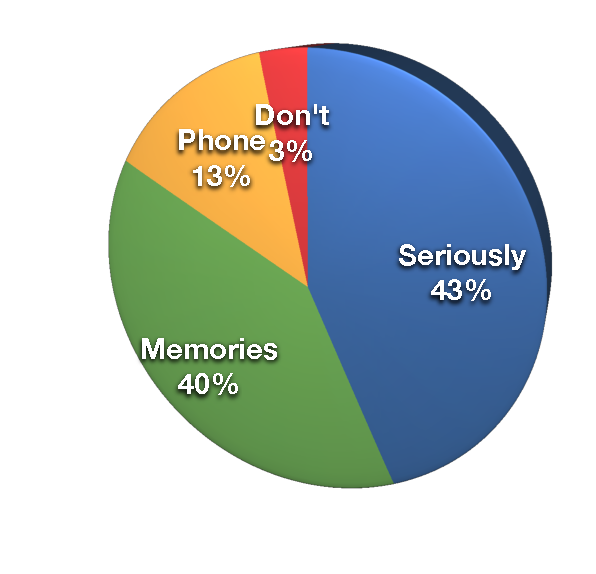
\includegraphics[width=\linewidth]{Figures/survey/desc}
	\end{center}
	\vspace{-20pt}
	\caption{Kinds of photographers.}
	\vspace{-5pt}
	\label{fig:us:desc}
\end{wrapfigure}

We asked the respondents what of the following options described them the best:

\begin{myitemize}
	\item I'm a \textbf{professional} photographer.
	\item I like to take photography \textbf{seriously} but I'm no professional.
	\item I like to take pictures just to keep as \textbf{memories}, but I'm not a photo-geek.
	\item I only use my camera \textbf{phone} for fun.
	\item I \textbf{don't} take pictures.
\end{myitemize}

As we can see on \fig{us:desc}, most respondents like photography and take photos, being mostly people who take photos for memories and people who are really into photography but are not professionals.

% subsubsection subsubsection_name (end)





\subsubsection{Storage of digital photos} % (fold)
\label{ssub:storage_of_digital_photos}
The second question was a check to verify if the respondents stored digital photos in their computers. The questionnaire would end if they said no. Fortunately, everyone said yes.
% subsubsection storage_of_digital_photos (end)





\section{Characterization of Photo Library} % (fold)
\label{sec:characterization_of_photo_library}

\begin{wrapfigure}{r}{0.5\textwidth}
	\vspace{-20pt}
	\begin{center}
		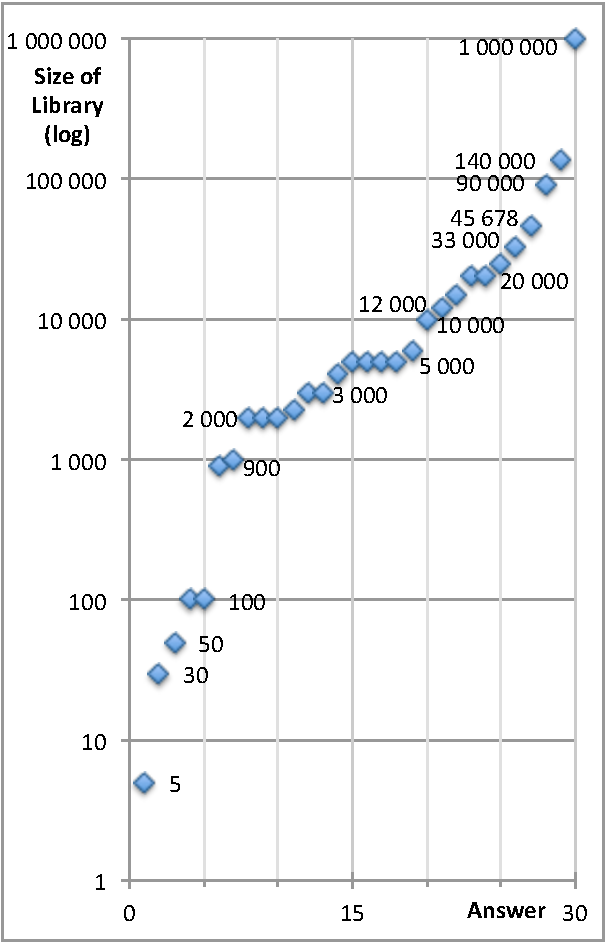
\includegraphics[width=\linewidth]{Figures/survey/libsize}
	\end{center}
	\vspace{-20pt}
	\caption{Library Size}
	\vspace{-70pt}
	\label{fig:us:desc}
\end{wrapfigure}

We then inquired about their photo libraries.
\vspace{\baselineskip}

\subsubsection{Library size} % (fold)
\label{ssub:library_size}

To start the survey about the library, we inquired how large was the respondents photo library.

We made this an open question, because we wanted to obtain real values from the users and not just limiting to a number of options that hardly represent anything. The answers for this question can be seen on \fig{us:desc}.

We were surprised by the values we got, going from 5 up to a million photos.

Almost half of the answers are between the 1 \nolinebreak 000 and the 10 000 values, having two thirds of the results falling between 0 and 10 000. We also found the median value of the answers, which is 5 \nolinebreak 000.

% subsubsection library_size (end)


\vspace{3\baselineskip}

\begin{wrapfigure}{r}{0.3\textwidth}
	\vspace{-20pt}
	\begin{center}
		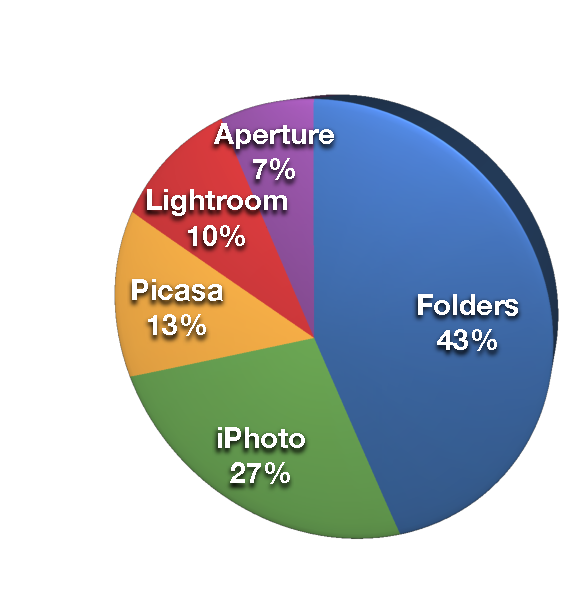
\includegraphics[width=\linewidth]{Figures/survey/sw}
	\end{center}
	\vspace{-20pt}
	\caption{Software used}
	\vspace{-5pt}
	\label{fig:us:desc}
\end{wrapfigure}

\subsubsection{Usage of Software} % (fold)
\label{ssub:usage_of_software}

We then questioned about what software applications did people use to help them organize their collections. Almost half admitted they only used folders for their organization, while the other 17 people used some kind of software.

Going through each software applications, we can see that 40\% use an entry-level software (iPhoto and Picasa) while 17\% prefer more Pro-level systems.

We tried to correlate the size of the collections with the software used but we realized that we probably don't have enough data for some of those softwares and that users might not have their entire collection inside the application, therefore defeating the correlation.

% subsubsection usage_of_software (end)

\pagebreak


\subsubsection{Systematic Organization} % (fold)
\label{ssub:systematic_organization}

\begin{wrapfigure}{r}{0.25\textwidth}
	\vspace{-20pt}
	\begin{center}
		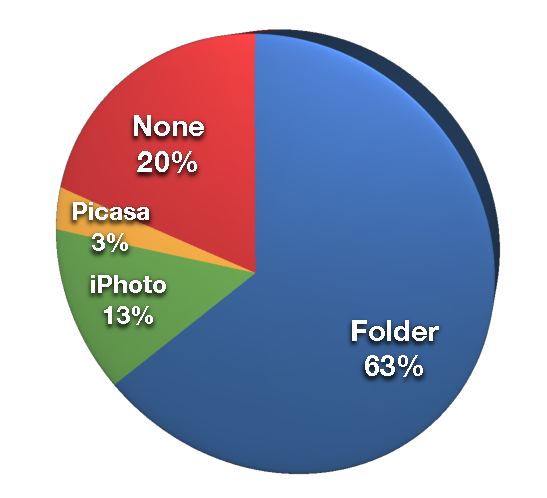
\includegraphics[width=\linewidth]{Figures/survey/organization}
	\end{center}
	\vspace{-20pt}
	\caption{Systematic organization in folders, in an application or no organization.}
	\vspace{-5pt}
	\label{fig:us:org}
\end{wrapfigure}

The question ``Do you have a systematic way to keep your photos organized?'' is meant to understand if people keep a system for their library, either on folders of inside an application.

Since most of the applications in the last question rely on folder organization, is no surprise that having a system in place for keeping things organized in folders is the clear winner of this question. Five people answered that they have this system inside an application and correlating this question with the previous one we found another expected aspect: only entry-level software is used to keep everything tidy, without touching folders, more exactly four people say they use iPhoto and one says Picasa is his/her choice.

In contrast, 20\% of the respondents claimed not having a way to organize their collections. The median of the number of photos of this group of people is 1050, the lowest, when compared to the other groups, the ones who use applications and the ones who rely on folders, both with 5000 of median.

% subsubsection systematic_organization (end)



\subsubsection{Photos in Close Sequence} % (fold)
\label{ssub:photos_in_close_sequence}

\begin{wrapfigure}{r}{0.25\textwidth}
	\vspace{-50pt}
	\begin{center}
		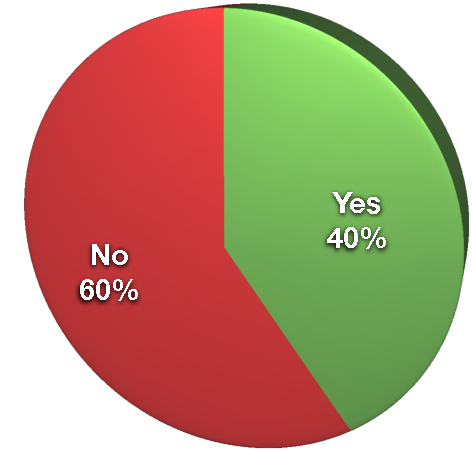
\includegraphics[width=\linewidth]{Figures/survey/close-seq}
	\end{center}
	\vspace{-20pt}
	\caption{Users that take photos in close sequence.}
	\vspace{-5pt}
	\label{fig:us:close-seq}
\end{wrapfigure}


% subsubsection photos_in_close_sequence (end)

The following question was intended to see how many users take photos in close sequence, e.g., bursts, panoramas, bracketing or time lapses, where the photographer ends up with many photos in a few seconds.

As we can see on \fig{us:close-seq}, 40\% of the respondents said they do take photos in close sequence. We also saw that this group has a median value of library size of 8000, whereas the other group stays on the 2150 images. In fact, of the total 13 enthusiasts, 11 of them answered yes on this question, followed by someone who claims only to take photos for memories.



\subsubsection{Preferred Features} % (fold)
\label{ssub:preferred_features}

\begin{wrapfigure}{r}{0.45\textwidth}
	\vspace{-50pt}
	\begin{center}
		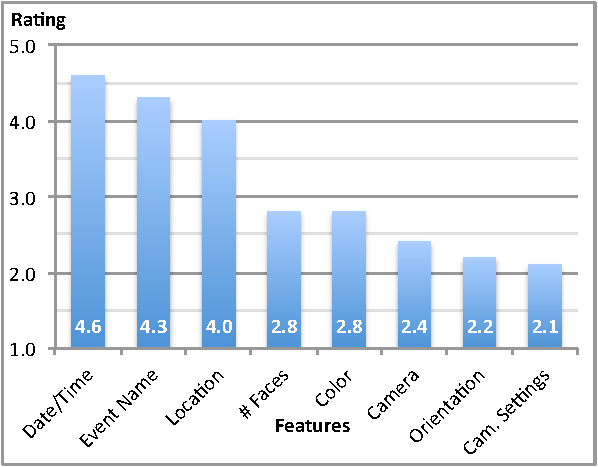
\includegraphics[width=\linewidth]{Figures/survey/features}
	\end{center}
	\vspace{-20pt}
	\caption{User rated features.}
	\vspace{-5pt}
	\label{fig:us:features}
\end{wrapfigure}

We had some ideas of what we would like to see extracted from the images and exposed to the user via our application and we asked for people's opinion on this survey and the results can be seen on \fig{us:features}.

While we weren't surprised by the favorites\linebreak Date/Time, Event and Location, we did expect\linebreak some higher ratings for number of faces and colors. Orientation and camera settings got the ratings we did expect.

% subsubsection preferred_features (end)



\subsubsection{Suggestions of Features} % (fold)
\label{ssub:suggestions_of_features}

In line with the previous question, we asked what other features they would like to see extracted from images.

\begin{itemize}
	\item The most common request, with about four different people requesting it, is people recognition. This allows photos to be tagged with the names of people in the photo and not just how many faces there are on the photo.

	\item Someone asked that, from a set of similar photos (exemplified with friend group photos), pick the one that, e.g., is more clear, has a better color, more smiles, more open eyes.

	\item Metadata was requested by three people, e.g., EXIF metadata, tags, format (RAW/JPEG), if the photo is the original or the edited version, the number of duplicates, the location on disk.

	\item One person asked for identification of whether the photo was taken during the day or the night.

	\item Another person was interested in having information about objects, buildings or animals.
\end{itemize}


\subsubsection{General Overview} % (fold)
\label{ssub:general_overview}

\begin{wrapfigure}{r}{0.4\textwidth}
	\vspace{-20pt}
	\begin{center}
		\includegraphics[width=\linewidth]{Figures/survey/overview}
	\end{center}
	\vspace{-20pt}
	\caption{Whether people think they can get a good overview or not.}
	\vspace{-5pt}
	\label{fig:us:overview}
\end{wrapfigure}

To conclude the survey, we asked if the respondents feel they have the tools to have a good overview of their collection at the same time.

The answers to this question rose some uncertainty, due to their mixed views. Each person is different from the next and so are their requirements. For instance, some people considered iPhoto/Apertures's events or projects as good overview for the library, but others don't think the same way about it, claiming it is limiting. On \fig{us:overview}, is a summary of whether people think they can get a good overview or not, split by the applications (or lack of them) they use. Also included is a global percentage for comparison.

One thing we can be sure, though: those who use folders don't think they can get a good overview from them.


% subsubsection general_overview (end)

\vspace{\baselineskip}

With this we conclude our survey.
% subsubsection suggestions_of_features (end)



% section characterization_of_photo_library (end)



\cleardoublepage

 % file "Thesis_Appendix.tex"

% ----------------------------------------------------------------------
%  Bibliography
% ----------------------------------------------------------------------

% Include all references in .bib file, even non-cited ones...
\nocite{*}

% Produces the bibliography section when processed by BibTeX
%
% Bibliography style
% > entries ordered alphabetically
%\bibliographystyle{plain}
% > unsorted with entries appearing in the order in which the citations appear.
%\bibliographystyle{unsrt}
% > entries ordered alphabetically, with first names and names of journals and months abbreviated
%\bibliographystyle{abbrv}
% > entries ordered alphabetically, with reference markers based on authors' initials and publication year
%\bibliographystyle{alpha}
%
% Replacement bibliography styles provided by 'natbib' package
% (plainnat.bst, abbrvnat.bst, unsrtnat.bst )
% > entries ordered alphabetically
\bibliographystyle{acm}
% > unsorted with entries appearing in the order in which the citations appear.
%\bibliographystyle{unsrtnat}
% > entries ordered alphabetically, with first names and names of journals and months abbreviated
%\bibliographystyle{abbrvnat}
% > entries ordered alphabetically, with reference markers based on authors' initials and publication year
%\bibliographystyle{alpha}


% External bibliography database file in the BibTeX format
\cleardoublepage
\bibliography{Thesis_bib_DB} % file "Thesis_bib_DB.bib"
% Add entry in the table of contents as chapter
\addcontentsline{toc}{chapter}{\bibname}
\cleardoublepage

% ----------------------------------------------------------------------
\end{document}
% ----------------------------------------------------------------------

